\documentclass{sig-alternate-05-2015}

%\usepackage[sorting=none]{biblatex}
\usepackage[utf8]{inputenc}
\usepackage[T1]{fontenc}
\usepackage{lmodern}
\usepackage{balance}
\usepackage{stys/standalone}
\usepackage{stys/relsize}
\usepackage[caption=false, font=footnotesize]{subfig}

\usepackage{url}
\usepackage{ifthen}
\usepackage{cite}
\usepackage{xspace}
\usepackage{pgfplots}
\usepackage{algorithm}
\usepackage{algpseudocode}
\usepackage{enumitem}
%\usepackage[pdftex]{graphicx}
\graphicspath{{./figs/}}
\DeclareGraphicsExtensions{.eps,.jpeg,.png}
\usepackage{epstopdf}
\usetikzlibrary{bayesnet}
%\newcommand{\comment}[1]{}
\newcommand{\mf}[1]{\mathcal{#1}}
\newcommand{\var}[1]{{\ttfamily#1}}
\newcommand{\Tgran}{\emph{granularity($\mf T$)}\xspace}
\newcommand{\Ggran}{\emph{granularity($\mf G$)}\xspace}
\newcommand{\our}{\mbox{HLens}\xspace}
\newcommand{\tmlda}{\mbox{TM--LDA}\xspace}
\newcommand{\lda}{\mbox{LDA}\xspace}
\newcommand{\atam}{\mbox{ATAM}\xspace}
\newcommand{\tmatam}{\mbox{TM--ATAM}\xspace}
\newcommand{\tatam}{\mbox{T--ATAM}\xspace}
\newcommand{\change}{\mbox{change-point}\xspace}
\newcommand{\changes}{\mbox{change-points}\xspace}
\newcommand{\season}{\emph{\texttt{homogenous\- time\- period}}\xspace}
\newcommand{\seasons}{\emph{\texttt{homogenous\- time\- periods}}\xspace}
\newcommand{\competitor}{\emph{\texttt{competitor\- topic\- model}}\xspace}
\newcommand{\transition}{\emph{\texttt{transition\- matrix}}\xspace}
\newcommand{\selftransition}{\mbox{stable-topic}\xspace}
\newcommand{\selftransitions}{\mbox{stable-topics}\xspace}

\newcommand{\titleA}{On Harnessing Social Media for Flu Predictions}
\newcommand{\titleB}{How to stop being sick and start enjoying life}
\newcommand{\titleC}{Flu Catcher ! It's like Bird Catcher For Flus}
\newcommand{\titleD}{Health-Lens: Microscopic Ailment Modeling Using Social Media}
\newcommand{\titleE}{Health Monitoring on Social Media over Time}

\renewcommand{\algorithmicrequire}{\textbf{Input:}}
\renewcommand{\algorithmicensure}{\textbf{Output:}}

\DeclareMathOperator*{\argmin}{arg\!min}
\DeclareMathOperator*{\argmax}{arg\!max}
\setlistdepth{9}

\newlist{myEnumerate}{enumerate}{9}
\setlist[myEnumerate,1]{label=(\arabic*)}
\setlist[myEnumerate,2]{label=(\Roman*)}
\setlist[myEnumerate,3]{label=(\Alph*)}
\setlist[myEnumerate,4]{label=(\roman*)}
\setlist[myEnumerate,5]{label=(\alph*)}
\setlist[myEnumerate,6]{label=(\arabic*)}
\setlist[myEnumerate,7]{label=(\Roman*)}
\setlist[myEnumerate,8]{label=(\Alph*)}
\setlist[myEnumerate,9]{label=(\roman*)}

\begin{document}

\conferenceinfo{WWW'16}{Montr\'eal, Canada}

\title{\titleE}

\numberofauthors{1} 
\author{
% 1st. author
\alignauthor Sumit Sidana, Sihem Amer-Yahia, Massih-Reza Amini,\\ Marianne Clausel, Shashwat Mishra \\
       \affaddr{Univ. Grenoble Alps/CNRS}\\
       \affaddr{Grenoble, France}\\
       \email{firstname.lastname@imag.fr}
%% % 2nd. author				
%% \alignauthor Shashwat Mishra\\
%%        \affaddr{Univ. Grenoble Alps/CNRS}\\
%%        \affaddr{Grenoble, France}\\
%%        \email{shashwat.mishra@imag.fr}
%% % 3rd. author
%% \alignauthor Sihem Amer-Yahia\\
%%        \affaddr{Univ. Grenoble Alps/CNRS}\\
%%        \affaddr{Grenoble, France}\\
%%        \email{Sihem.Amer-Yahia@imag.fr}
%% % 4th. author
%% \alignauthor Marianne Clausel\\
%%        \affaddr{Univ. Grenoble Alps/CNRS}\\
%%        \affaddr{Grenoble, France}\\		
%%        \email{marianne.clausel@imag.fr}
%% \and  % use '\and' if you need 'another row' of author names
%% % 5th. author
%% \alignauthor Massih-Reza Amini\\
%%        \affaddr{Univ. Grenoble Alps/CNRS}\\
%%        \affaddr{Grenoble, France}\\
%%        \email{massih-reza.amini@imag.fr}
}
\maketitle

\begin{abstract}
Social media has become a major source for analyzing all aspects of
daily life. Thanks to dedicated latent topic analysis methods such as
the Ailment Topic Aspect Model (\atam), public health can now be
observed on Twitter. In this work, we are interested in using social
media to monitor people's health over time and enable a range of
applications such as measuring behavioral risk factors and triggering
health campaigns.  Recently, Temporal-LDA (\tmlda) was proposed for
efficiently modeling general-purpose topic transitions over time. In
this paper, we propose Temporal Ailment Topic Aspect (\tmatam), a new
latent model dedicated to capturing transitions that involve
health-related topics.  \tmatam learns topic transition parameters by
minimizing the prediction error on topic distributions between
consecutive posts at different time and geographic granularities. We then 
go on to propose \tatam, where time is treated as a random variable inside the \atam. Our
experiments on an 8-month corpus of tweets show that \tmatam
outperforms \tmlda in estimating transitions involving health-related
topics for different geographic populations. We then examine
the ability of \tmatam to determine transitions due to different
factors such as climate, nutrition and lifestyle. Additionally, we compare the results
 of \tatam with Center of Disease Control.
\end{abstract}

\category{H.4}{Information Systems Applications}{Miscellaneous}
%\category{J.4}{SOCIAL AND BEHAVIORAL SCIENCES}
\terms{Experimentation, Performance}
\keywords{public health, ailments, social media, topic models} 

\section{Introduction}
Social media has become a major source of information for analyzing
all aspects of daily life. In particular, public health monitoring can
now be conducted on Twitter in order to measure the wellbeing of
populations in different geographic regions. The ability to model
transitions for ailments and detect statements such as ``people talk
about smoking and cigarettes before talking about respiratory
problems'', or ``people talk about headaches and stomach ache in any
order'', has a range of applications in syndromic surveillance such as
measuring behavioral risk factors and triggering public health
campaigns. In this paper, we propose \tmatam, a method that models
temporal transitions that involve health-related topics. \tmatam
combines \atam, a latent health-related topic analysis method proposed
in~\cite{atam2}, with \tmlda, that models general-purpose topic
transitions~\cite{DBLP:conf/kdd/WangAB12}. We then propose \tatam,
a method which uncovers latent ailment inside tweets by treating
\texttt{\emph{time}} as a random variable inside
atam~\cite{atam2}.

Common ailments are continuously monitored by collecting data from
health care facilities, a process known as sentinel surveillance. Such
resources limit surveillance, most especially for real-time
feedback. For this reason, the Web has become a source of syndromic
surveillance, operating on a wider scale for a fraction of the
cost. While several latent topic modeling methods such as
Probabilistic Latent Semantic Indexing (pLSI)~\cite{plsi} and Latent
Dirichlet Allocation (LDA)~\cite{lda}, are used to effectively cluster
and classify general-purpose text, it has been shown that dedicated
methods such as the Ailment Topic Aspect Model (ATAM) are better
suited for capturing ailments in
Twitter~\cite{atam2}. ATAM extends LDA to model how users
express ailments in tweets. It assumes that each health-related tweet
reflects a latent ailment such as flu and allergies.  Similar to a
topic, an ailment indexes a word distribution. It also maintains a
distribution over symptoms and treatments. This level of detail
provides a more accurate model for latent ailments.

\begin{figure*}[t!]
\centering
\frame{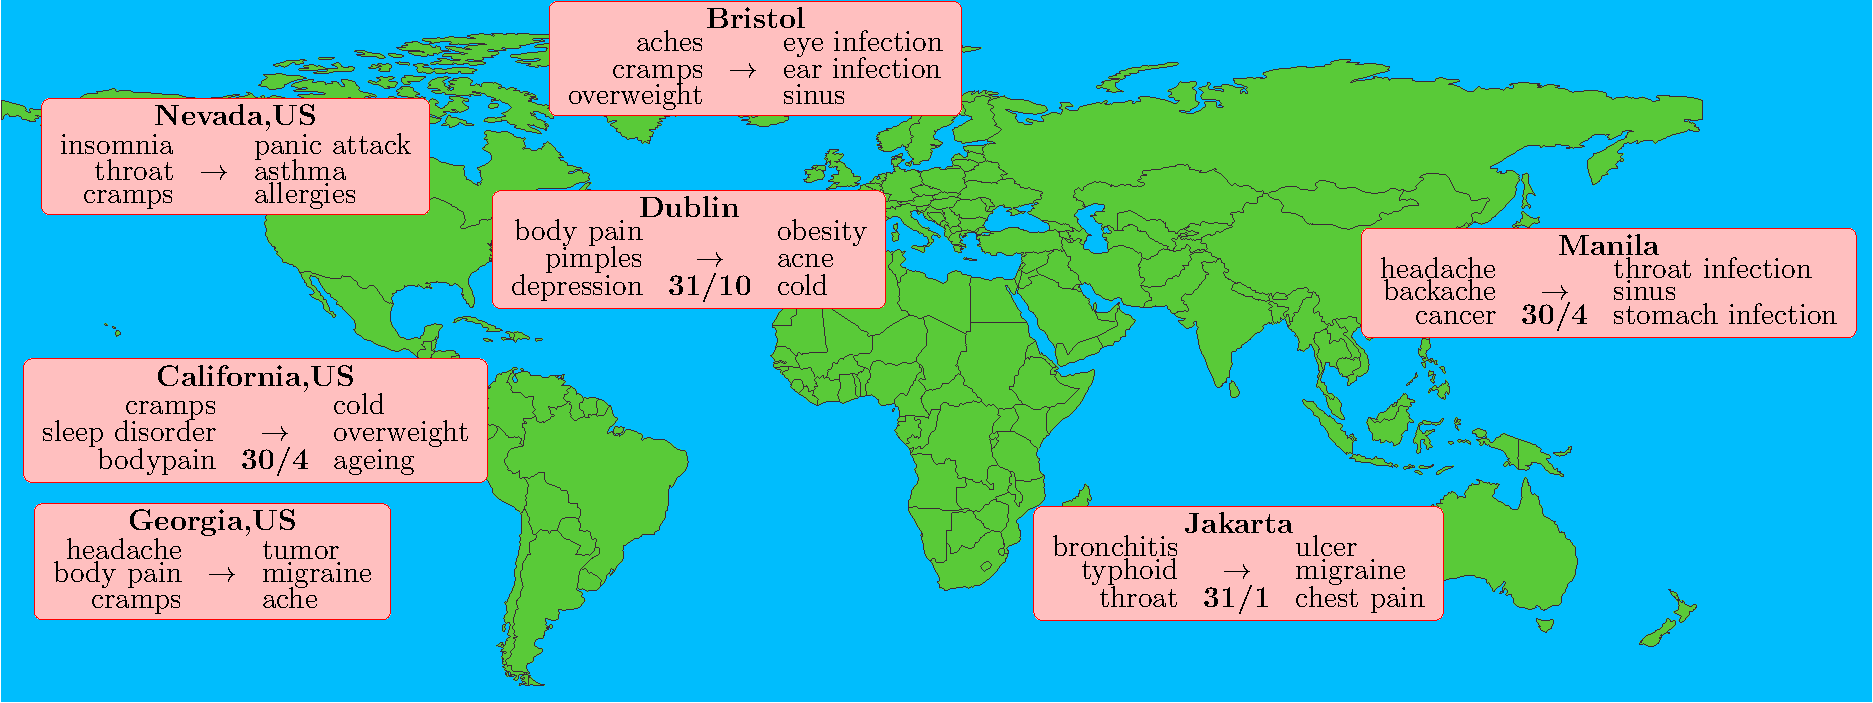
\includegraphics[width=0.80\textwidth]{tikz/eyecatcher.pdf}}
\caption{One-Way ailment transitions obtained by \tmatam for various 
regions. For each location the time period is divided into two parts, 
preceding and following the most significant change-point discovered
for that location. We show the most popular ailments on either 
side of this boundary.}
\label{fig:eyecatcher}
\end{figure*}

On the other hand, while pLSI and LDA have been shown to perform well
on static documents, they are not able to intrinsically capture topic
evolution over time.  Temporal-LDA (\tmlda) was hence proposed as an
extension to LDA for mining Twitter streams and providing effective
topic prediction over time~\cite{DBLP:conf/kdd/WangAB12}. In this
paper, we examine how well we can measure and predict ailment
transitions in Twitter by combining ATAM and TM-LDA into a new model,
coined \tmatam.  Just like \tmlda, \tmatam and \tatam are different from dynamic
topic models such as~\cite{DBLP:conf/icml/BleiL06}
and~\cite{DBLP:conf/icdm/LinMHJD11}, and from the work of Wang et
al.~\cite{DBLP:conf/kdd/WangM06}, as they are designed to learn topic
transition patterns from temporally-ordered posts, while dynamic topic
models focus on changing word distributions of topics over
time. \tmatam learns transition parameters that dictate the evolution
of health-related topics by minimizing the prediction error on ailment 
distributions of consecutive periods at different temporal and geographic 
granularities. \tatam on the other hand discovers latent ailments
in health tweets by treating time as a corpus-specific multinomial distribution.

Ailment distributions evolve over time. Further the evolution is
region-specific. While \tmatam and \tatam heavily borrow from ATAM and \tmlda,
their effectiveness require to carefully model two key granularities,
temporal and geographic. A temporal granularity that is too-fine may result in
sparse and spurious transitions whereas a too-coarse one could miss
valuable ailment transitions. Similarly, a too-fine geographic
granularity may produce false positives and a too coarse one may cover
a user population that is exposed to different weather conditions and
miss meaningful transitions. For example, it has been shown that discussions on
allergies break at different periods in different states in the
USA~\cite{atam2}. Therefore, processing all tweets originating from the USA together
will miss climate variations that affect people's health. We argue
for the need to consider different time granularities for different
regions and we wish to identify and model the evolution of ailment
distributions between different temporal granularities.

Our experiments on a corpus of more than $500K$ health-related tweets
collected over a period of 8 months show that \tmatam outperforms
\tmlda in estimating temporal topic transitions of different
geographic populations. Our results can be classified in 2 kinds of
transitions. {\selftransitions} are those where a health-related topic
is mentioned continuously. {\em One-Way transitions} cover the case where
some topics are discussed after others. For example, our
study of tweets from California revealed many self transitions such as
headaches and migraines. On the other hand, tweeting about smoking,
drugs and cigarettes is followed by tweeting about respiratory
ailments. Figure~\ref{fig:eyecatcher} shows example one-way transitions we extracted for different states and cities in the
world. Such transitions are often due to external factors such as climate, health campaigns, nutrition and lifestyle of different world populations.

The outline of the paper is as follows: in
Section~\ref{sec:background} we first introduce the key ingredients of 
our data model, and then present the necessary background on
topic modeling (\lda, \atam). Finally we formalize the ailment prediction
problem. In Section~\ref{sec:approach}, we describe the construction of \tmatam and \tatam.
In Section~\ref{sec:results} we present the experiments designed to study
the behavior and performance of \tmatam and \tatam. Related work is overviewed in 
Section~\ref{sec:relwork}. We conclude and give some perspectives for 
future work in Section~\ref{sec:conclusion}.

\section{Data model and problem}
\label{sec:background}
We first define a model that maps tweet posts to documents of
different time and geographic granularities. We then review the
principles of general-purpose topic modeling with LDA~\cite{lda} and
health-related topic modeling with \atam~\cite{atam2}. We conclude this
section with our problem definition.

\subsection{Mapping Tweets to Documents}
\begin{table}[b!]
\centering
\caption{Mapping tweets to documents}
\label{tab:model:terms}
\begin{tabular}{|c|c|}
\hline
{\bf Term} & {\bf Description}\\
\hline
$\mf P$ & posts\\
\hline
$\mf G$ & regions\\
\hline
$\mf T$ & time periods\\
\hline
$\mf P_g^t$ & posts from region $g$ during time $t$\\
\hline
$D_g^t$ & document-set built by mapping the content\\
& of each post $p\in \mf P_g^t$ to a document\\
\hline
\end{tabular}
\end{table}

We consider a set of posts $\mf P=\{p_1,p_2...p_n\}$. A \emph{post} 
is the smallest unit of user-activity on a social media platform, 
such as a tweet, a tumblr post, or a facebook status update. In 
addition to a unique identifier and content, we assume the existence 
of two attributes, geographic coordinates and timestamp, for each
post, $<id,\ coord,\ tstamp,\ content>$.

Let $\mf G=\{g_1,g_2,...\}$ represent a set of geographic regions 
around the world. We use $\mf P_g$ to refer to the set of posts 
in $\mf P$ that originate from a region $g \in \mf G$. The choice 
of a geographic granularity (country, state, county) is required 
to instantiate $\mf G$.

In similar fashion, with a suitable choice of temporal granularity, 
we could divide up the entire time range spanned by posts in $\mf P$ into 
{\em disjoint and consecutive} periods, $\mf T=\{t_1,t_2...\}$. 
Possible choices for instantiation of $\mf T$ are week, bi-week, 
month, etc. We use $\mf P_g^t$ to refer to the set of posts in
$\mf P$ that originated from a region $g$ during period $t$.
% \comment{
% 	\begin{equation}
% 		\label{eq:pgt}
% 		\mf P_g^t=\{p|p\in \mf P,\ p.coord \in g,\ p.tstamp\in t\}
% 	\end{equation}
% }
We consider a set of documents $D_g^t$ formed by mapping the content 
of each post in $P_g^t$ to a document. We use 
$\mf D=\{D_g^{t_1},D_g^{t_2},\ldots\}$ to denote all document-sets 
corresponding to tweets from region $g$ for different time periods in $\mf T$.

Table~\ref{tab:model:terms} presents a summarized
version of the terminology associated to our work.

\subsection{Uncovering Latent Topics in Tweets}
We now review the principles of general-purpose topic modeling and
health-related topic modeling. Existing models are (generally)
unsupervised generative models that describe document content in a
large document collection $D$. In our case, $D$ corresponds to
$D_g^t$, the set of documents built from tweets originating from 
region $g$ during time period $t$. 

\subsubsection{Uncovering Latent Topics with LDA}
Latent Dirichlet Allocation (LDA) represents each document as
a probability distribution over $k$ topics~\cite{lda}. Each topic 
in turn $z$ is represented as a probability distribution over a set of
words. LDA assumes that the topic distribution $\theta_d$ of a 
document $d$ and the vocabulary distribution $\phi_z$ of a 
topic $z$ are generated according to a Dirichlet distribution. 
Vectorial parameters $\alpha$ and $\beta$ of the Dirichlet distribution
are assumed to be common to the corpus.

While LDA is successful at uncovering generic topics such as
``healthcare'', ``obesity'', ``substance abuse'' infrequent topics 
that may be related to specific subjects, such as the
topic ``tobacco use'', pose a challenge to LDA. Furthermore, for an
excessively frequent topic, such as ``weight loss'', LDA adds noise,
in the form of words such as ``gardening'', ``oils'', ``anti-ageing'', 
``muscle gain'', that are not related to the topic~\cite{atam2,prier2011identifying}.
Due to such limitations, LDA is not a good choice for modeling latent topics
present in health--related data.

\subsubsection{Uncovering Health Topics with \atam}
The probabilistic \emph{Ailment Topic Aspect Model} was designed 
specifically to uncover latent health-related topics present in a 
collection of tweets~\cite{atam2}. The proposed method achieves
remarkable improvement over LDA in discovering topics that correspond to 
ailments (in addition to discovering general topics). The novelty 
of \atam is that it distinguishes {\em background words} 
such as ``home'' and ``watching TV'' from {\em health-related words} 
such as ``hurts'' and ``allergy''. For each document, 
these health--related words are considered to correspond to a unique 
ailment such as ``obesity'',``insomnia'' or ``injuries''.
The word could be associated to the ailment as its symptom 
(e.g., the word ``weight'' is clearly a symptom related to the ailment
``obesity''), a treatment (the word ``diet'' is clearly a symptom
related to the ailment ``obesity'') or a general word (the word
``dentist'' is not a background word and belongs to the vocabulary of
the ailment ``dental'' but is neither a symptom nor a treatment).

% \comment{
% 	\begin{itemize}
% 	\item Set the background switching binomial $\lambda$
% 	\item Draw an ailment distribution $\eta\sim Dir(\sigma)$
% 	\item Draw word multinomials $\phi\sim Dir(\beta)$ for the topic, ailment,  and background distributions
% 	\item For each message $1 \leq m \leq D$
% 	\begin{itemize}
% 	\item Draw a switching distribution $\pi\sim Beta(\gamma_0,\gamma_1)$
% 	\item Draw an ailment $a \sim Mult(\eta)$
% 	\item Draw a topic distribution $\theta \sim Dir(\alpha_a)$
% 	\item For each word $w_i \in  N_m$
% 	\begin{itemize}
% 	\item Draw aspect $y_i\in\{0,1,2\}$ (observed)
% 	\item Draw background switcher $\ell\in\{0,1\} \sim Bi(\lambda)$
% 	\item If $\ell == 0$~: Draw $w_i \sim Mult(\phi_{B,y})$ (a background)
% 	\item Else:
% 	\begin{itemize}
% 	\item Draw $x_i \in\{0,1\}\sim Be(\pi)$
% 	\item If $x_i == 0$ (draw word from topic $z$)~:Draw topic $z_i \sim Mult(\theta)$ and word $w_i \sim Mult(\phi_z)$.
% 	\item Else: (draw word from ailment $a$, aspect $y$)~: Draw $w_i\sim Mult(\phi_{a,y})$
% 	\end{itemize}
% 	\end{itemize}
% 	\end{itemize}
% 	\end{itemize}
% }

When generating a document (tweet), one first
associates to it an ailment such as ``allergy'', ``insomnia'' or
``injury''. Thereafter, the document is generated word by
word. Using the random variables $\ell$ and $x$, one chooses if the
word is a background word or a general-purpose word ($\ell=0$ or $\ell=1,x=0$). The word can be
drawn from a vocabulary distribution common to the whole corpus (case
$\ell=0$) or generated from a LDA-type (from an underlying Dirichlet distribution)
 topic $z$ (case $\ell=1,x=0$). When the
word is related to health (case $\ell=1,x=1$), the random variable $y$
enables to choose if this word is a aspect-neutral (case $y=0$), a
symptom (case $y=1$) or a treatment (case $y=2$). Words are hence
drawn depending on the ailment $a$ which has been associated to the
document. The topic distribution vector for a sample tweet is shown 
in Figure~\ref{fig:ldavsatam}. Note the stronger relevance to 
health--related matters in this vector than in the topic distribution vector 
generated by LDA for the same tweet. 
\begin{figure}[t!]
\centering
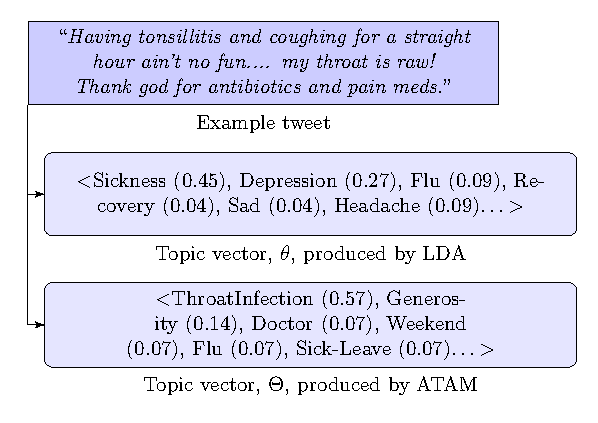
\includegraphics[width=0.45\textwidth]{tikz/exampleTweet1.pdf}
\caption{\lda vs \atam: Comparison of topic distributions for an example tweet.}
\label{fig:ldavsatam}
\end{figure}

\subsubsection{Topic Evolution Over Time}
\begin{figure}[b!]
\centering
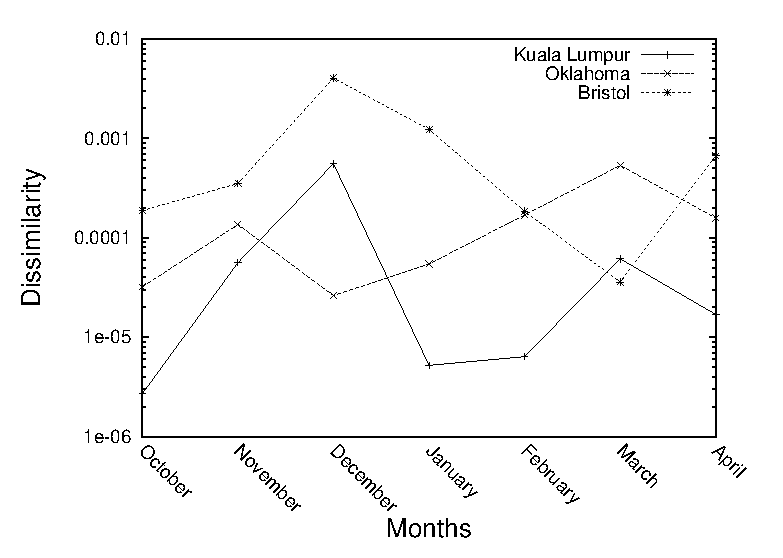
\includegraphics[width=0.45\textwidth]{gnuplot/distributiondifference/bhattacharyadistance.eps}
\caption{Topic transitions over time.}
\label{fig:ailmentsEvolve}
\end{figure}

We convert inferences of \atam over a single document to associate with a given set of documents $D_g^t$, an ailment
distribution, $\Theta_g^t$. $\Theta_g^t$ is a mix of general-purpose and health-related topics.
 $\Theta_g^t$ is a vector over a set of latent ailments where the weight of each ailment is representative of 
the ailment's occurrence in the tweets originating from region $g$ 
during period $t$. 


Ailment distributions evolve over time. Further the evolution is
region-specific as the spread of ailments is heavily influenced by the
weather and by socio-economic factors. For a region $g$, the interval
of time spanning a set of consecutive time periods
$\{t_i,t_{i+1},\ldots\}$ during which discovered ailment distributions 
$\{\Theta_g^{t_i},\Theta_g^{t_{i+1}},\ldots\}$
do not change appreciably forms a \texttt{\emph{\season}} w.r.t. ailments. By definition, a \season is (nearly) homogeneous in terms
of ailments. In other words, the ailments evolve in a smooth fashion
within a \season and change abruptly across \season boundary. We posit that such \seasons exist after which they encounter \changes in ailment topic discussions.
These \changes in ailment topic discussions 
may be caused by onset of the disease or some other external factors.
Nevertheless, they are the interesting points for analyzing purposes.

As an example, in Figure~\ref{fig:ailmentsEvolve}, we show the difference
between ailment distributions of consecutive months for 3 different
regions Kuala Lumpur (a city in Indonesia), Oklahoma (a state in
the USA), and Bristol (a city in the UK). The sharp peaks obtained
validate the existence of time intervals that are homogeneous w.r.t. ailments.

Note that a high weight for ailment $a$ in the distribution $\Theta$
only indicates that people tend to tweet about $a$ 
and need not necessarily imply
that people suffer from $a$. High weight can be attributed to a number 
of factors. For example, if a health awareness campaign on Amyotrophic 
Lateral Sclerosis 
(ALS)~\footnote{\url{https://en.wikipedia.org/wiki/Amyotrophic_lateral_sclerosis}} 
is organized in region $g$ during period $t_i$, the 
weight of ALS in $\Theta_g^{t_i}$ would be significantly higher than 
in $\Theta_g^{t_{i-1}}$ or $\Theta_g^{t_{i+1}}$ as the ailment would
appear more frequently in the tweets during period $t_i$. 
%% \begin{figure}[htpb]
%% \centering
%% \includegraphics[width=0.4\textwidth]{tikz/model.pdf}
%% \caption{\tmatam work model.}
%% \label{fig:model:tmatam}
%% \end{figure}

\subsection{Ailment prediction problem}
\label{subsec:problem-general}
We are now ready to define our problem in its general form. A more
precise form of this problem will be given in Section~\ref{subsec:problem}. 
Given a set of documents $D_g^{t_{i-1}}$ formed by tweets originating 
from a region $g \in G$ during time period $t_{i-1}$, predict the 
topic distribution of documents in $D_g^{t_i}$, corresponding to 
posts from $g$ in period $t_i$ from the topic distribution of 
document $D_g^{t_{i-1}}$ corresponding to posts from $g$ during 
period $t_{i-1}$.

Note that this problem statement does not distinguish between
general-purpose topics and health-related topics.

\section{Our model and approach}
\label{sec:approach}
We now develop our model and use it to specify our problem more
precisely. We then present our algorithm to address our ailment
prediction problem.

\subsection{General-purpose topic modeling over time with \tmlda}
To take into account the evolution of the underlying topics of a
dynamic collection of documents with time (e.g., a microblog or a
facebook page) Wang et al. (2012) introduced a modified version of the
LDA model, \tmlda~\cite{DBLP:conf/kdd/WangAB12}.
In ~\cite{DBLP:conf/kdd/WangAB12}, \tmlda was introduced to extend
lda with modeling topic evolution of dynamic collection of documents over time
 Topic distribution
of the $i$--th document, $\theta_i$  is ascertained from 
the topic distribution of the previous document, $\theta_{i-1}$.
At the heart of the algorithm lies the following equation.
\begin{equation}
	\label{eq:tmlda:basic}
	\theta_{i}\approx\frac{\theta_{i-1}.M}{\|\theta_{i-1}.M\|_{\ell_1}}
\end{equation}
where $M$ is a $k\times k$ matrix, called the transition
matrix, and $k$ is the number of topics. To obtain the transition matrix, 
the authors propose to solve the following least square
problem ($\|\cdot\|_F$ denotes the Frobenius norm and X denotes the search space):
\begin{equation}
	\label{eq:tmlda:train}
	M=\argmin_X{\|A.X-B\|_F}
\end{equation}
where $A$ and $B$ are as specified below.
\begin{equation}
	\label{eq:tmlda:vectors}
	A=\begin{pmatrix}\theta_{1}\\\vdots\\\theta_{i-1}\end{pmatrix},\,B=\begin{pmatrix}\theta_{2}\\\vdots\\\theta_{i}\end{pmatrix}
\end{equation}
However, while being quite elegant in modeling general purpose topics
\tmlda is not specialized to capture \texttt{\emph{health}} transitions
over time.
\subsection{\tmatam: Modeling Health Topics over Time}
\label{subsec:model}
While \atam is effective at modeling health-related topics, 
it is not designed to model topic transitions over time. 
We hence propose \tmatam that builds on top of \atam and \tmlda. 
\tmatam computes the aggregate topic distribution, $\Theta_g^t$, 
of a set of documents $D_g^t$. Qualitatively, the topic distribution 
has the following components. 
\begin{itemize}
\item $\eta_g^t$ : Distribution over ailments in $D_g^t$
\item $\theta_g^t$ : Distribution over general topics in $D_g^t$
\item $\Theta_g^t=\begin{pmatrix}(1-\pi)\theta_g^t& \pi\eta_g^t\end{pmatrix}$ 
where $\pi$ is the proportion of non-health words related to some 
aspect of an ailment. We show $\Theta$ for an example tweet in 
Figure~\ref{fig:exampleTweet2}.
\end{itemize}
\begin{figure}[b!]
\centering
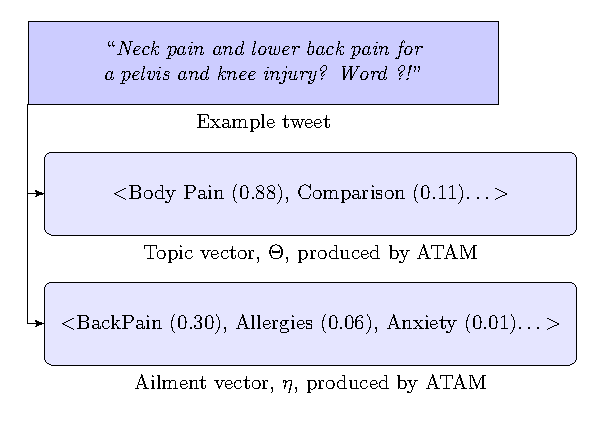
\includegraphics[width=0.45\textwidth]{tikz/exampleTweet2.pdf}
\caption{$\Theta$ predicted by \atam on an example tweet, while $\eta$ predicted by ATAM on region containing example tweet}
\label{fig:exampleTweet2}
\end{figure}

\tmatam, at its heart, solves following equation.
\begin{equation}
A_g^{t}\approx A_g^{t-1}.M
\end{equation}
where
\begin{equation}
A_g^{t-1}=\begin{pmatrix}\Theta_g^1\\\vdots\\\Theta_g^t\end{pmatrix},\,A_g^t=\begin{pmatrix}\Theta_g^2\\\vdots\\\Theta_g^{t+1}\end{pmatrix}%d_g^{t-1}=\begin{pmatrix}P_1\\\vdots\\P_t\end{pmatrix},\,d_g^t=\begin{pmatrix}P_2\\\vdots\\P_{t+1}\end{pmatrix}
\end{equation}
$M$ is an unknown transition matrix which is obtained by solving the following least square problem.
\[
\min_M\|A_g^t- A_g^{t-1}.M\|_F
\]
\tmatam thus learns a transition matrix which is used to model health topics.

\subsection{Ailment prediction problem revisited}
\label{subsec:problem}
We are now ready to revisit our problem: Given a set of
documents $D_g^{t_{i-1}}$ formed by tweets originating from a region
$g \in G$ during time period $t_{i-1}$, predict $\eta_g^{t_i}$, the
ailment distribution of documents in $D_g^{t_i}$, corresponding to
posts from $g$ in period $t_i$ from $\Theta_g^{t_{i-1}}$, the ailment
distribution of document $D_g^{t_{i-1}}$ corresponding to posts from
$g$ during period $t_{i-1}$.  Our framework can predict $\eta_g^{t_i}$, $\theta_g^{t_i}$ or $\Theta_g^{t_i}$
 but in our experiments, we found  using $\Theta_g^{t_{i-1}}$ to predict $\eta_g^{t_i}$ is the most interesting to our cause.  

\subsection{Algorithm}
\label{subsec:tmalg}
Algorithm~\ref{alg:tmatam} contains the steps of our solution. It has 
two main parts: {\texttt{\emph{ \change detection}}} and {\texttt{\emph{ ailment prediction}}}. 
We first describe how \changes are detected then we show how ailment topics being discussed in twitter 
are predicted over time within \seasons.

\paragraph{\change Detection}
We use $\mf Z$ to refer to the set of all health-related and non-health 
related topics. For each region $g \in \mf G$ (Line~\ref{alg:line:start}) 
we first run \atam over the full time period $D_g$ (Line~\ref{alg:line:atam}).
Next for each period $t\in \mf T$ (Line~\ref{alg:line:tstart}), 
we use the output of \atam over $D_g$ to generate 
topic distribution $\Theta_g^t$ (Lines~\ref{alg:line:createThetaStart}--
\ref{alg:line:createThetaEnd}). 
Note that, $\Theta_g^t$ includes general-purpose topics as well as ailments that are
discussed in tweets originating from region $g$ during time period $t$.  
% \comment{
% \begin{figure}[b!]
% \centering
% \includegraphics[width=0.45\textwidth]{tikz/Thetaatam.pdf}
% \caption{$\Theta_{atam}$ - Topic distribution vector as predicted by ATAM on a tweet}
% \label{fig:atamTheta}
% \end{figure}
% \begin{figure}[b!]
% \centering
% \includegraphics[width=0.45\textwidth]{tikz/ThetaatamContrast.pdf}
% \caption{$\Theta_{atam}$ - Topic distribution vector as predicted by ATAM on a second tweet}
% \label{fig:atamTheta2}
% \end{figure}
% } 
Next we examine the distance between consecutive distributions
$\Theta_g^{t-1}$ and $\Theta_g^t$ of the region $g$ 
to identify the most significant \texttt{\emph{\change}}, $t_c$ (Line~\ref{alg:line:ThetaDiff}).
We treat the choice of distance measure $m$ as black box, 
which could be \emph{Bhattacharya Distance}\footnote{\url{https://en.wikipedia.org/wiki/Bhattacharyya_distance}} or \emph{Cosine Similarity}\footnote{\url{ https://en.wikipedia.org/wiki/Cosine_similarity}}. 
The time period $t_c$ is termed as the \texttt{\emph{\change}} for
region $g$. The entire span of time, $[t_1\ t_{|\mf T|}]$, is divided 
into two intervals, \emph{pre}, consisting
of all time periods prior to the \emph{\change} (Line~\ref{alg:line:buildSeasonPre}), 
and \emph{post}, consisting of all time periods after 
the \emph{\change} (Line~\ref{alg:line:buildSeasonPost}).

We term these intervals as \seasons w.r.t ailments being discussed in twitter. Qualitatively, \season is a 
time interval (collection of consecutive time periods) during which
the tweets originating from the region are homogeneous in terms of ailment topics. 
The \texttt{\emph{\change}} characterizes a significant change point
in the evolution of ailments. We posit that such change points exist. These change points in ailment topic discussions
may be caused by onset of the disease or some other external factors. Nevertheless, they are the interesting points for analyzing purposes.
Such analysis may lead to various insights into onset of diseases.
Onset of disease is usually affected by several factors, such as weather, which may cause
a sudden onslaught of ailments different from the ones that were in circulation
previously. The pervasive nature of communicable diseases is also a contributing
factor. Note that the results in Figure~\ref{fig:ailmentsEvolve} support our assumption.

\paragraph{Ailment Prediction}
The key idea in \tmatam is to identify \emph{\changes} and predict
evolution of topics within each \season. This is a fresh departure
from existing solutions that operate in a \season-agnostic fashion.
By definition, a \season is (nearly) homogeneous in terms
of ailments. In other words, the ailments evolve in a smooth fashion
within a \change and change abruptly across \change boundaries.
In this study, we limit ourselves to finding a single \change boundary for
each region $g$. While this may not be true for all regions, we obtain
significant improvement in terms of prediction accuracy over the previous
state of the art with just a single boundary.
We outline in lines~\ref{alg:line:predStart}--\ref{alg:line:predEnd} 
of Algorithm~\ref{alg:tmatam} the steps undertaken. 
\begin{algorithm}[t]
\caption{TM-ATAM: \change Detection and Training Ailment Distribution Predictor}
\label{alg:tmatam}
\begin{algorithmic}[1]
 \ForAll {$g \in G$}\label{alg:line:start}
 \State Run ATAM on $D_g$\label{alg:line:atam}
 \ForAll  {$t \in \mf T$}:\label{alg:line:tstart}
 \ForAll {$z \in \mf Z$}:\label{alg:line:createThetaStart}
 \State $\Theta_g^t[z] \leftarrow 0$
 \EndFor
 \ForAll {$d \in D_g^t$}:
 \ForAll {$w \in d$}:
 \State $z \gets topic(w)$
 \State $\Theta_g^t[z] \gets \Theta_g^t[z] + \frac{1}{|d|\times |D_g^t|}$
 \EndFor
 \EndFor\label{alg:line:createThetaEnd}
 \EndFor
 \State $\displaystyle t_{c} = \argmax_t{\ m(\Theta_g^{t-1},\ \Theta_g^{t})}$\label{alg:line:ThetaDiff}
 \State $pre = [t_1\ ,\ t_{c-1}]$\label{alg:line:buildSeasonPre} 
 \State $post = [t_{c}\ , \ t_{|\mf T|}]$\label{alg:line:buildSeasonPost} 
 \ForAll {$s \in \{pre,\ post\}$}:\label{alg:line:predStart}
 \State $A_g^t\approx A_g^{t-1}.M$
 \State $M =(A_g^{t-1\intercal}A_g^{t-1})^{-1}A_g^{t-1\intercal}A_g^t$
 %\State $M = A_g^{t-1}\textsuperscript{\textdagger}A_g^t=(A_g^{t-1\intercal}A_g^{t-1})^{-1}A_g^{t-1\intercal}A_g^t$
 \EndFor\label{alg:line:predEnd}
\EndFor\label{alg:line:end}
\end{algorithmic}
\end{algorithm}

\subsection{Time-Aware Ailment Topic Aspect Model (T-ATAM)}

\begin{figure}[ht]
  \begin{center}
    \documentclass[a4paper]{article}

\usepackage{tikz}
\usetikzlibrary{bayesnet}
\title{Time-Aware Ailment Topic Aspect Model}
% \author{Sumit Sidana}

\begin{document}

\maketitle

  % Define nodes
  \begin{tikzpicture}[x=1.7cm,y=4.8cm]
  % Nodes

  \node[obs]                   (word)      {$w$} ; %
  \node[latent, left=3cm of word] (background) {$l$};
  \node[latent, above=1cm of background] (route) {$x$};
  \node[obs, right=1cm of route]    (aspect)      {$y$} ; %
  \node[latent, right=2.5cm of aspect]    (topic)  {$z$}; %
  \node[latent, above=2cm of word] (ailment) {$a$};
  \node[obs, left=1.5cm of ailment] (timestamp) {$t$};
  \node[latent,above=0.3cm of topic] (theta){$\theta$};
  \node[latent,above=0.3cm of route] (pi){$\pi$};
  \node[latent,left=1cm of background](lambda){$\lambda$};
  \node[latent,above=0.5cm of ailment](eta){$\eta$};
  \node[latent,left=0.5cm of eta](sigma){$\sigma$};
  \node[latent,above=0.5cm of pi](gamma){$\gamma$};
  \node[latent,above=0.5cm of timestamp](psi){$\psi$};
  \node[latent,above=1cm of psi](mu){$\mu$};
  \node[latent,above=1cm of theta](alpha){$\alpha$};
 
%   \node[const, above=of topic] (atheta) {$\alpha_\theta$};
  
\edge {background,route,aspect,topic,ailment} {word} ;
\edge {ailment}{timestamp}
\edge {theta}{topic}
\edge {pi}{route}
\edge {lambda}{background}
\edge {eta}{ailment}
\edge {sigma}{eta}
\edge {gamma}{pi}
\edge {psi}{timestamp}
\edge {mu}{psi}
\edge {alpha}{theta}

  \plate {plate1} {(word)(background)(route)(aspect)(topic)} {$N$} ;
  \plate {} {(word)(background)(route)(aspect)(topic)(ailment)(timestamp)(theta)(pi)(plate1)}{$D$};
  \plate {} {(mu)}{$A$}
  \plate {} {(alpha)}{$A$}
  % Factors
%   \factor[above=of X]     {X-f}     {Multi} {} {} ; %
%   \factor[above=of T]     {T-f}     {left:Multi} {} {} ; %
%   \factor[above=of theta] {theta-f} {left:Dir} {} {} ; %

  % More nodes
%   \node[latent, right=of X-f] (phi)  {$\phi$}; %
%   \node[const, above=of phi]  (aphi) {$\alpha_\phi$}; %

%   \factor[above=of phi] {phi-f} {right:Dir} {} {} ; %

%   \factoredge {theta}  {T-f}     {T} ; %
%   \factoredge {atheta} {theta-f} {theta} ; %
%   \factoredge {phi}    {X-f}     {X} ; %
%   \factoredge {aphi}   {phi-f}   {phi} ; %
% 
%   \gate {X-gate} {(X-f)(X-f-caption)} {T}

%   \plate {plate1} { %
%     (X)(X-gate) %
%     (T)(T-f)(T-f-caption) %
%   } {$\forall 1 \leq i \leq n_d$}; %
%   \plate {} { %
%     (plate1) %
%     (theta)(theta-f)(theta-f-caption) %
%   } {$\forall d \in \mathcal{D}$} ; %
%   \plate {} { %
%     (phi)(phi-f)(phi-f-caption) %
%   } {$\forall t \in \mathcal{T}$} ; %
  \end{tikzpicture}
% TikZ examples for graphical models (Bayesian networks) and directed
% factor graphs \cite{Dietz:2010}.
\end{document}

  \end{center}
  \caption{Time-Aware Ailment Topic Aspect Model.}
\label{T_atam}
\end{figure}

%\begin{figure}[t!]
%\centering
%\frame{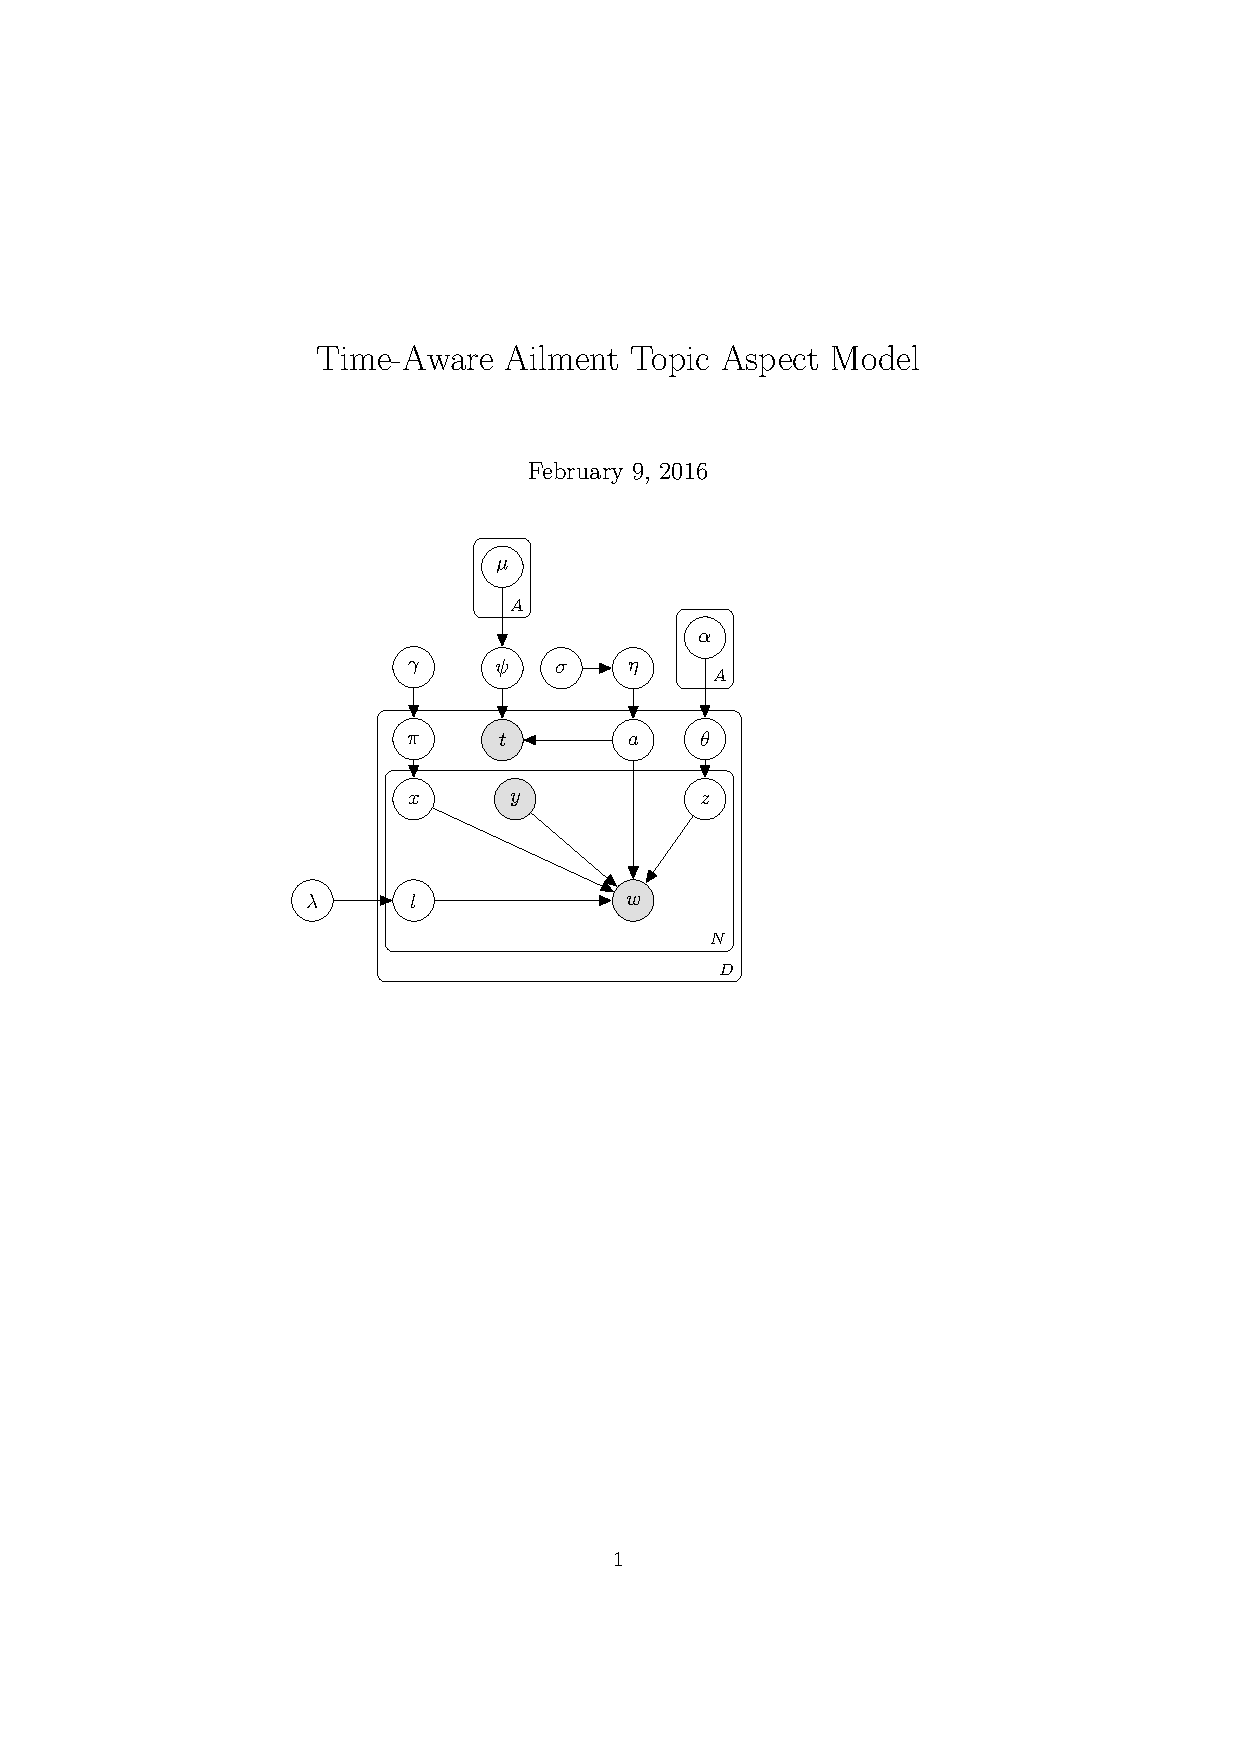
\includegraphics[width=0.45\textwidth]{tikz/plate.pdf}}
%\caption{Time-Aware Ailment Topic Aspect Model.}
%\label{T_atam}
%\end{figure}
\paragraph{Generative Process}
\begin{myEnumerate}
 \item Set the background switching binomial $\lambda$
 \item Draw an ailment distribution $\eta \sim Dir(\sigma)$ 
 \item Draw A multinomials $\psi_A \sim Dir(\mu)$
 \item Draw word multinomials $\phi \sim Dir(\beta)$ for the topic, ailment, and background distributions
 \item For each message $1\ \leq m\leq D$
 \begin{myEnumerate}
  \item Draw a switching distribution $\pi \sim Beta(\gamma_0,\gamma_1)$
  \item Draw an ailment $a\sim Mult(\eta)$
  \item Draw a time stamp $t \sim Mult(\psi_a)$
  \item Draw a topic distribution $\theta \sim Dir(\alpha_a)$
  \item For each word $w_i\in N_m$
  \begin{myEnumerate}
   \item Draw aspect $y_i\in\{0,1,2\}$(observed)
   \item Draw background switcher $l\in\{0,1\}\sim Bi(\lambda)$
   \item if l == 0:
   \begin{myEnumerate}
    \item Draw $w_i\sim Mult(\phi_{B,y})$(a background)
   \end{myEnumerate}
   \item Else:
   \begin{myEnumerate}
    \item Draw $x_i\in \{0,1\} \sim Bi(\pi)$
    \item If $x_i == 0:$(Draw word from topic z)
    \begin{myEnumerate}
     \item Draw topic $z_i\sim Mult(\theta)$
     \item Draw $w_i \sim Mult(\phi_z)$
    \end{myEnumerate}
    \item Else:(draw word from ailment a aspect y)
    \begin{myEnumerate}
     \item Draw $w_i \sim Mult(\phi_{a,y})$
    \end{myEnumerate}
    
        \end{myEnumerate}

   \end{myEnumerate}
   


  \end{myEnumerate}


\end{myEnumerate}

\section{Experimental evaluation}
\label{sec:results}
We conduct experiments to evaluate the performance of \tmatam on 
real world data. We present our results as follows. 
Section~\ref{subsec:summary} highlights the key insights drawn 
from our experiments. Section~\ref{subsec:setup} describes the 
experimental setup including the datasets and test-bench. In 
Section~\ref{subsec:perf1}, we compare \tmatam against previous 
state-of-the-art approaches. That is followed by a detailed study of
the behavior of \tmatam in Section~\ref{subsec:perf2}. Finally, 
a qualitative analysis of \tmatam's results in Section~\ref{subsec:qualitative}.

\begin{figure}[t!]
\centering
\frame{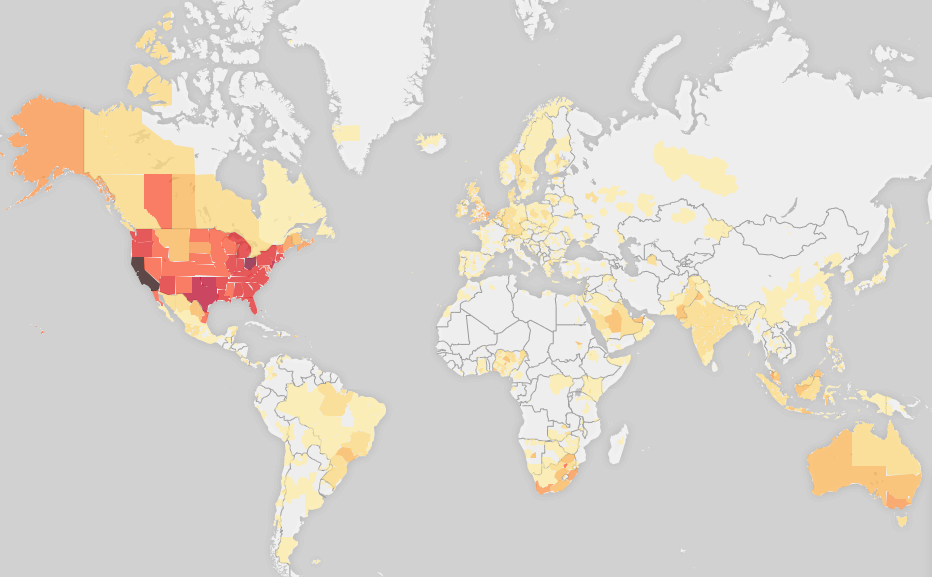
\includegraphics[width=0.45\textwidth]{heatmap/heatmap}}
\caption{Heatmap over collected health tweets. A major fraction
of the tweets originate from various states in the US.}
\label{fig:data:heatmap}
\end{figure}

\subsection{Summary of results}
\label{subsec:summary}
By modeling transitions in the same \change, TM–ATAM
consistently outperforms \tmlda in predicting 
health topics in all social-media active regions.

We analyze the performance of \tmatam by changing spatio-temporal parameters.
In particular, we find that prediction accuracy for health topics is higher when operating \tmatam on finer spatial granularity and shorter time periods.

Further, we go on to discover interesting region-specific intra and inter-\change health-related transitions. 
While studying these transitions, we find that \changes are continuous time periods for which people in the same region tweet about similar health issues. When those \changes end, we found that ailments discussed in Twitter transition into other ailment topics.
These results show that it is more logical to predict future ailments concerning people within the same \change of a
region than on any random health tweets.

By outperforming \tmlda in predicting future health topics, we show that it is essential 
to use a dedicated method that separates health-related topics from other topics. 

\begin{table}
\centering
\caption{Dataset Statistics}
\label{tab:data:stats}
\begin{tabular}{|c||c|}
\hline
collection period (days) & 235\\
\hline
\#tweets & {1,360,705,803}\\
\hline
\#tweets (health-related) & 698,212\\
\hline
\#tweets (health-related+geolocated) & 569,408\\
\hline
\end{tabular}
\end{table}
\subsection{Setup}
\label{subsec:setup}
\subsubsection{Data}

We employ Twitter's Streaming API to collect tweets. We use the \emph{Decahose Stream}\footnote{\url{https://dev.Twitter.com/streaming/overview}} which gives a $10\%$ random sample of the total tweets generated 
each day. We collect tweets for the period $2014$-Oct-$8$ to $2015$-May-$31$.
The collected tweets were subjected to two preprocessing steps described next.

{\bf Filtering health-related tweets:} Since our interest lies 
in public health discourse on social media, we filter the tweets 
returned by the \emph{Decahose Stream} to obtain \emph{health-related} 
tweets. We say that a tweet is health-related if it has a health 
keyword and passes our classification criteria.
The process is automated with the help of an SVM classifier
 ~\cite{DBLP:journals/ml/CortesV95}
with linear kernel and uni-gram, bi-gram and tri-gram word 
features. To this end, a modest-sized sample of the original 
corpus was annotated through crowdsourcing efforts where annotators 
were asked to label $5128$ tweets. The precision and recall of the 
employed classifier are $0.85$ and $0.44$. Table~\ref{tab:data:stats} 
shows that out of the 1.36B tweets we collected, 689K were health-related. 

{\bf Geolocation:} The ability to operate seamlessly at varying 
geographic resolutions mandates that the exact location of each 
tweet be known to \tmatam. Twitter affords its users the option 
to share their geolocation. It has been shown that a very small 
number of Twitter users choose to share their location. While 
this artefact results in significant reduction in the number of 
tweets, in absolute terms, we retain more than half a million 
tweets ($569K$ as indicated in Table~\ref{tab:data:stats}). 
% \comment{
% 	Note that recently, the problem of automated geotagging of tweets 
% 	has drawn attention of the research community and several solutions 
% 	have been proposed. In this work, we refrain from using any such 
% 	strategy and use a simple filtering scheme to retain tweets that 
% 	could be geolocated. 
% }
In Figure~\ref{fig:data:heatmap}, we present a heatmap that shows 
the geographic spread of these tweets. The darker the color, 
the higher the number of tweets. The top-10 regions (at spatial 
granularity \emph{state}) with the highest number of health tweets 
lie exclusively in the US.

\subsubsection{Test-Bench}
We run our experiments on a {32 core Intel Xeon @ 2.6Ghz CPU 
(with 20MB cache per core)} system with {128 Gig} RAM running 
{Debian GNU/Linux 7.9 (wheezy)} operating system.
All subsequently discussed components were implemented in 
Java {1.8.0\_60}.

\subsection{\tmatam vs \tmlda}
\label{subsec:perf1}
% \comment{
% 	\subsubsec{\change Detection at geographic granularity state and temporal granularity month}
% 	\label{subsubsec:season2}
% 	We first observe that it is unlikely for a county to exhibit health 
% 	patterns independent and different from its neighboring counties. 
% 	We hence decide to operate at the state level and obtain $1938$ states, 
% 	but not all of them are active tweeters on health. We choose to 
% 	filter only those \textit{active states} with at least one tweet 
% 	per week for the entire time period. We get 66 such active states. 
% 	We run ATAM~\cite{atam2} on health tweets of each state and convert its
% 	output into $monthly$ distributions as described in Algorithm~\ref{alg:tmatam}. 
% 	We do not choose to instantiate with $week$ as weekly distributions 
% 	were found to be too sparse. Our distribution vectors consist of 
% 	both ailment topics and general-purpose topics. We compute the 
% 	Bhattacharya Distance between topic distributions of
% 	consecutive months. The month-pair with the highest distance is 
% 	termed as \textit{change point} and the time period
% 	before and after the \textit{change point} are termed as $\changes$ 
% 	as defined in Section~\ref{sec:background}. Figure~\ref{fig:ailmentsEvolve}
% 	shows December to January as the \textit{change point}s for Kuala Lumpur. 
% }

\subsubsection{Perplexity Measure}
\begin{table}[t!]
\centering
\caption{Default Parameters}
\label{tab:parameters}
\begin{tabular}{|c|c|c|}
\hline
{\bf Term} &{\bf Description} & {\bf Value}\\
\hline
$\mf G$ &Geographic granularity &\emph{states}\\
\hline
$\mf T$ &Temporal granularity &\emph{months}\\
\hline
$m$ &Distance measure&\emph{Bhattacharya}\\
\hline
\end{tabular}
\end{table}
We use \emph{perplexity}, an empirical measure often used in NLP.
\footnote{\url{https://en.wikipedia.org/wiki/Perplexity}}
Perplexity of a language model measures how accurately the model can 
explain previously unseen data/documents. Given a language model
$l$ and a document $d$, perplexity is defined as below.
\begin{equation}
        \label{eq:perplexity}
	Perplexity(l) = 2^{-\sum_{w_i\in d} \log p_l(w_i)}
\end{equation}
This formula of perplexity for a document $d$ can be converted to a formula of perplexity for a set of documents $D_g^t$ as follows:
\begin{equation}
        \label{eq:perplexityGeoTemp}
	Perplexity\_{D_g^t}(l) = 2^{-\sum_{w_i\in d} \log \frac{\sum_{d\in D_g^t}p_l(w_i)}{|D_g^t|}}
\end{equation}
Formula \ref{eq:perplexityGeoTemp} denotes the perplexity of language model $l$ on a document-set at geo-granularity $g$ and temporal granularity $t$. 
Higher probability of words that occur in unseen documents results in lower perplexity and is hence better.
Here, $p_l(w_i)$ is the probability of occurrence of word $w_i$ as 
estimated by the language model $l$ in the document set. Previously unseen words can result in infinite perplexity. We use add-one smoothing to overcome this fact \footnote{\url{https://en.wikipedia.org/wiki/Additive_smoothing}}.
We compute perplexity of \tmatam and then compare perplexity of \tmatam with that of \tmlda on the same test document set  $D_g^t$ as explained in the next section. Both \tmatam and \tmlda are treated as  language models
as both give out probability of each word for any document-set $D_g^t$.
% \comment{
% 	\begin{figure}[t!]
% 	\centering
% 	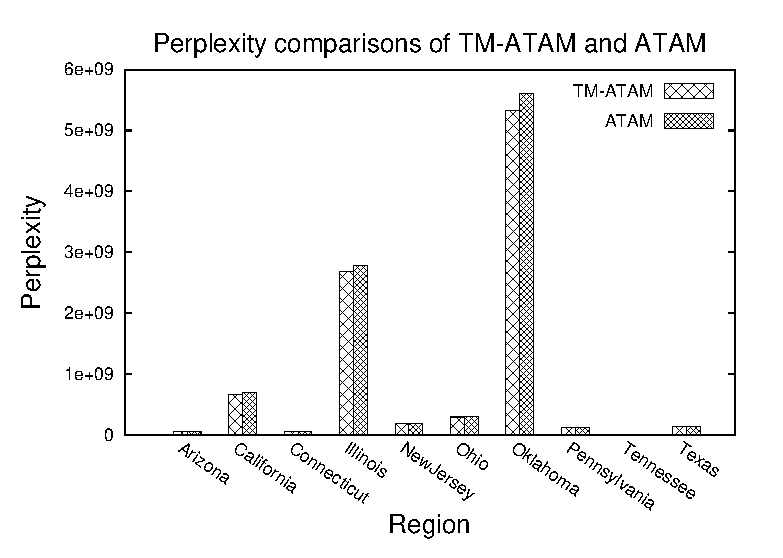
\epsfig{file=gnuplot/perplexity/perplexityAtamUS,width=0.45\textwidth}
% 	\caption{\tmatam and \atam prediction accuracies for top-10  active US states.}
% 	\label{fig:perplexityAtam}
% 	\end{figure}
% 	\begin{figure}[t!]
% 	\centering
% 	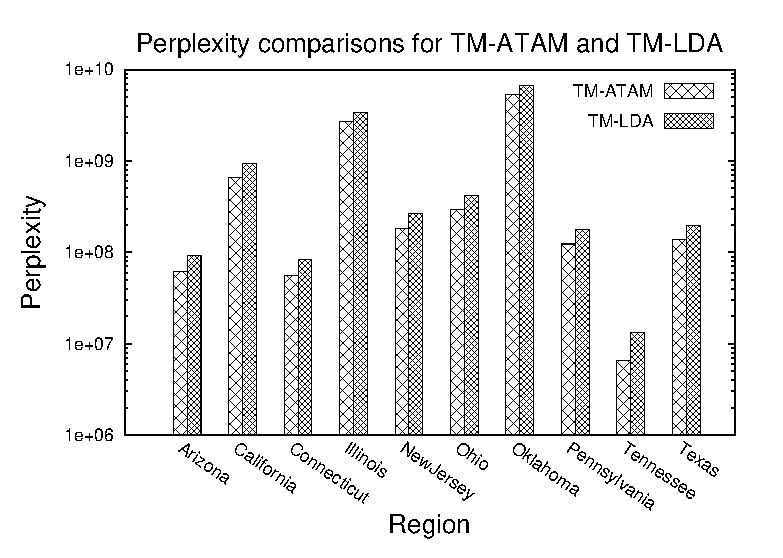
\epsfig{file=gnuplot/perplexity/perplexityUS,width=0.45\textwidth}
% 	\caption{\tmatam and \tmlda prediction accuracies for top-10  active US states.}
% 	\label{fig:perplexity1}
% 	\end{figure}
% 	\begin{figure}[t!]
% 	\centering
% 	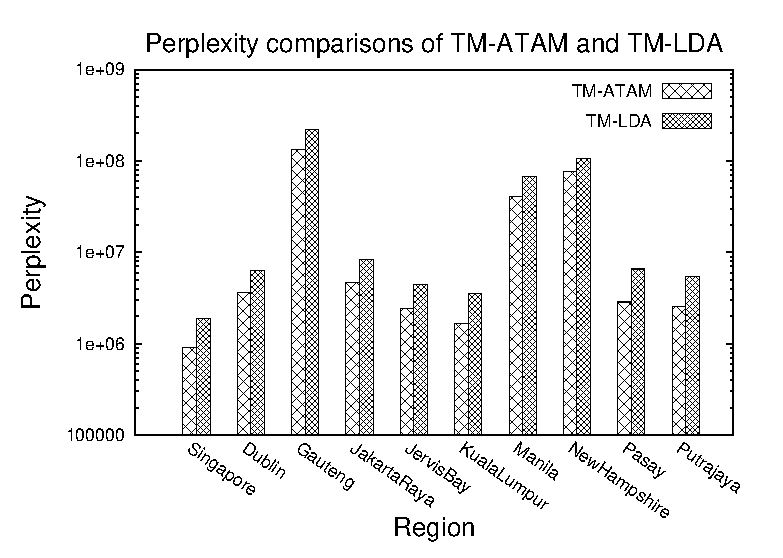
\epsfig{file=gnuplot/perplexity/perplexityNonUS,width=0.47\textwidth}
% 	\caption{\tmatam and \tmlda prediction accuracies for top-10 active non-US states.}
% 	\label{fig:perplexity2}
% 	\end{figure}
% }

\begin{figure*}[t!]
\centering
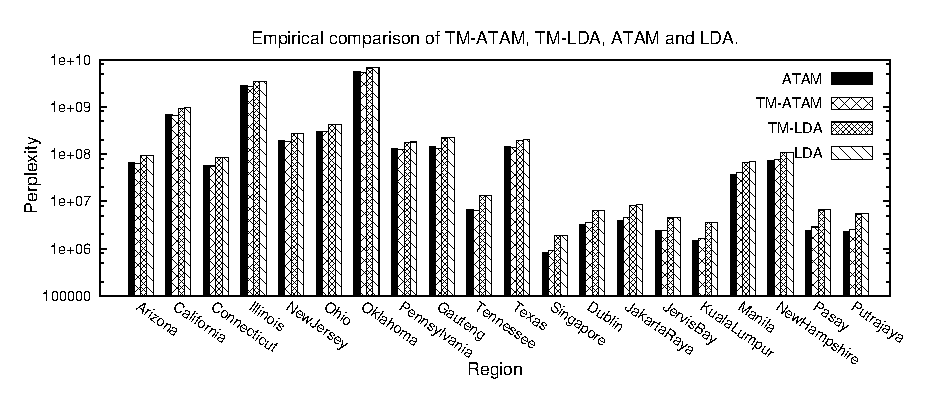
\epsfig{file=gnuplot/perplexity/perplexity,width=0.95\textwidth}
\caption{Perplexity comparison of \tmatam,\tmlda and \atam for top 20 social media active regions.}
\label{fig:perplexity}
\end{figure*}

\subsubsection{Comparing \tmatam with \tmlda and \atam}
We present results on the comparison of prediction accuracy of \tmatam
against \tmlda. We first divide the postings of each region into two 
\changes as inferred by $t_{c}$. We then divide each \change into train and test set as follows.
$Pre$-\change is divided into  train $([t_1\ ,t_{c-3}])$ and test $([t_{c-2},t_{c-1}])$ set. $post$-\change is divided into
train $([t_{c+1},t_{|\mf T|-2}])$ and a test $([t_{|\mf T|-1},t_{|\mf T|}])$ set. For example, if $t_c$ for a region is between January to February, then train set and test set of $pre$-\change are tweet posts of the months in the set [October,December] and [January,February] respectively. Train and test set of $post$-\change are tweet posts of months in the set [March,April] and  [May,June] respectively.
 We obtain 69 \changes for 66 regions. ATAM is \textit{re-run} over train set of each \change. It should be noted that though computing \textit{change point $t_c$} required access to full dataset, perplexity calculations are done within each \change and clear distinction is made between train and test set while computing it.  We then model a transition matrix 
$M_{tmatam}$ on the training data of each \change as described in Section~\ref{subsec:tmalg}. 
For each tweet $p$ of the first month in the test set $(t_{c-2}$ for the $pre$ \change and $t_{|\mf T|-1}$ for the $post$ \change), 
we compute the probability of "health topic" $z$ using the following formulas: \\
\begin{equation}
\label{eq:probabilitytopicgiventimepre}
P(z|t_{c-2}) = \frac{\sum_{p\ over\ the\ t_{c-2}}P(z|p\ for\ t_{c-2} )}
    {number\ of\ tweets\ for\ t_{c-2}}
\end{equation}
\begin{equation}
\label{eq:probabilitytopicgiventimepost}
P(z|t_{|\mf T|-1}) = \frac{\sum_{p\ over\ the\ t_{|\mf T|-1}}P(z|p\ for\ t_{|\mf T|-1} )}
    {number\ of\ tweets\ for\ t_{|\mf T|-1}}
\end{equation}
 Here $P(z|p)$ is computed simply by ($w$ is the word of tweet $p$): \\
\begin{equation}
\label{eq:probabilitytopicgiventweet}
 P(z|p)=\sum_{w}P(z|w)P(w|p) = \sum_{w}\frac{n(z,w)}{n(w)}P(w|p)
\end{equation}
Here, values for $n(z,w)$,$n(w)$ are taken from ATAM run on the training months. If we encounter an unseen word, we use add-one smoothing to avoid $P(w|p)$  to shoot to infinity and hence perplexity to shoot to infinity. P(z|w) is simply the number of times word $w$
occurs in the tweet $p$ divided by the total number of words in the tweet $p$.
We then predict the future probability of each topic in the 
second month of the test data ($P(z|t_{c-1})$ for $pre$ \change and $P(z|t_{|\mf T|})$ for the $post$ \change) using the corresponding transition matrix $M_{tmatam}$. The perplexity of \tmatam can now be computed against the words of the tweets of second test month ($t_{c-1}$ and $t_{|\mf T|}$)  using the formula~\ref{eq:perplexityGeoTemp}. This gives 69 values of perplexity, 
one for each \change of each region. We compare our results with following competitors:
\begin{itemize}
\item \atam: In order to assert the fact that health topics transit from one to another, we compare performance of \tmatam with \atam by computing perplexity of \atam on words of first month of test set and not predicting any topic distribution using transition matrix. For each tweet p of the first month in the test set ($t_{c-2}$ for the $pre$ \change and $t_{|\mf T|-1}$ for the $post$ \change), we compute the probability of "health topic" z using the formulas \ref{eq:probabilitytopicgiventimepre},\ref{eq:probabilitytopicgiventimepost},\ref{eq:probabilitytopicgiventweet}. It should be noted that in this case \textit{we do not model a transition matrix to predict probability of topics for second month of test set}. Hence, this denotes model where health topics stay \textit{static}. We can then compute perplexity of \atam against words of actual tweets of the first months of test month $(t_{c-2}$ and $t_{|\mf T|-1}$).  As shown in figure \ref{fig:perplexity}, \tmatam beats \atam in all US active regions. In Non-US active regions, the performance of \tmatam gets affected due to no substantial change in health topics with time.
\item Predicted \tmlda: Each region can be viewed as a 
\texttt{virtual user} and the transition matrix $M_{tmlda}$ of \tmlda is trained
by solving least squares problem in the following manner. We merge 
the training data of each \change in each region and train a transition
matrix of \tmlda. So, training data for \tmlda is the same as that of \tmatam: $([t_1\ ,t_{c-3}])$ for the $pre$ \change and $([t_{c+1},t_{|\mf T|-2}])$ for the $post$ \change.
% \comment{
% 	\begin{figure}[b!]
% 	\centering
% 	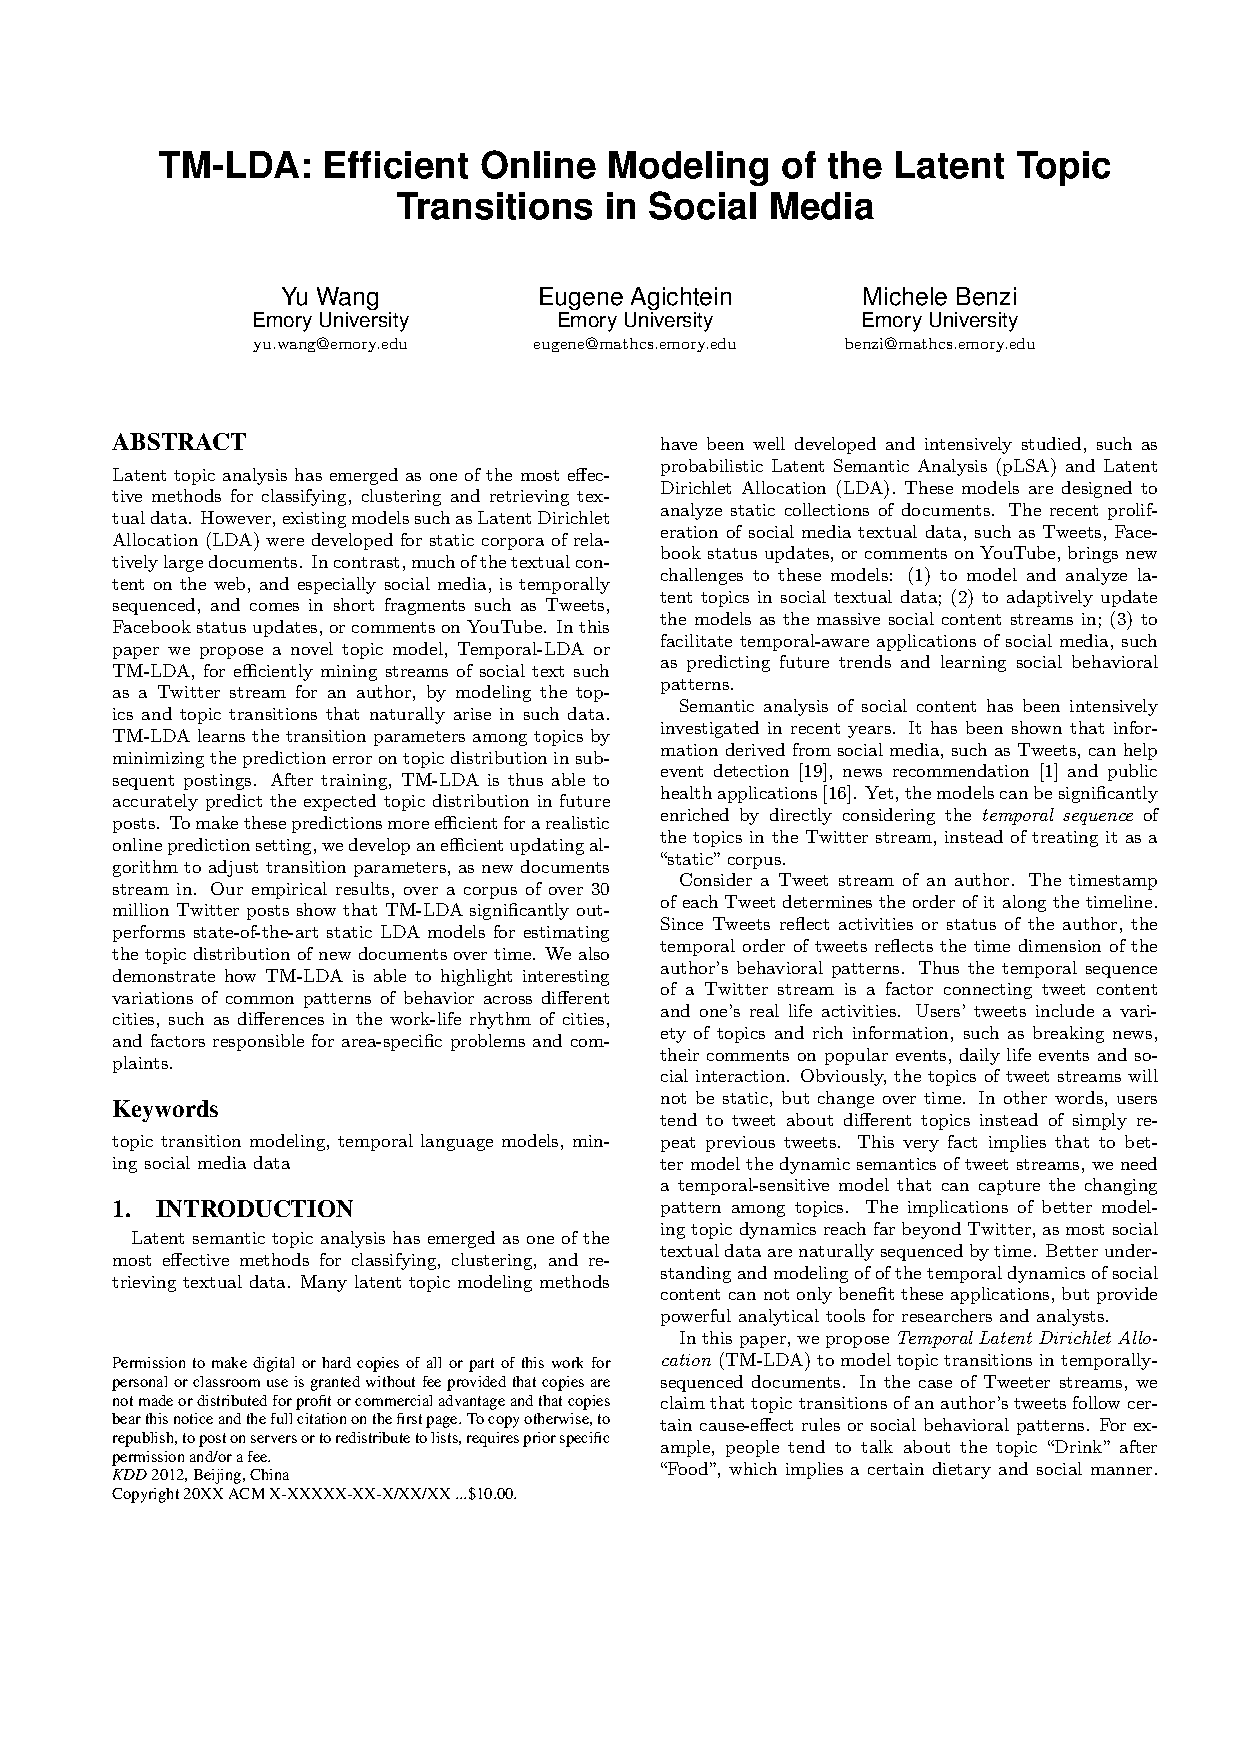
\includegraphics[width=0.45\textwidth]{tikz/tmlda.pdf}
% 	\caption{TM-LDA Model}
% 	\label{fig:tmlda}
% 	\end{figure}
% }
For each tweet $p$ of the first month of the test months $(t_{c-2}$ and $t_{|\mf T|-1}$), we compute the 
probability $P(z|t_{c-2})$ and $P(z|t_{|\mf T|-1})$ using LDA trained on merged training data (Formulas \ref{eq:probabilitytopicgiventimepre},\ref{eq:probabilitytopicgiventimepost},\ref{eq:probabilitytopicgiventweet}). We 
then predict the future probability of each topic in following month ($t_{c-1}$ and $t_{|\mf T|}$)
using corresponding $M_{tmlda}$. We can then compute the perplexity of \tmlda 
against words of actual tweets of the test months ($t_{c-1}$ and $t_{|\mf T|}$) using formula \ref{eq:perplexityGeoTemp} . 
\end{itemize}
$p_l(w_i)$, probability of word, for any document set is calculated as follows:
\begin{equation}
\label{eq:probabilityword}
p_l(w_i)=\sum_{z}P(w|z)P(z) = \sum_{z}\frac{n(z,w)}{n(z)}P(z)
\end{equation}
Here $P(z)$ is the probability of topic, which is computed by  multiplying corresponding transition matrix ($M_{tmatam}$ or $M_{tmlda}$) by the matrix formed during the training phase (\tmatam or \tmlda). Having computed P(w), we can compute perplexity using the formula \ref{eq:perplexityGeoTemp}. We take average over both \changes ($pre$ and $post$) and get a perplexity value for each region. 
Figures~\ref{fig:perplexity} and~\ref{fig:perplexity} show that \tmatam
consistently beats \tmlda in predicting
future health topics on the test month by computing lower perplexity on the words of the tweets of the test month in all social media active states.
\subsection{\tmatam: Effect of parameters}
\label{subsec:perf2}
\subsubsection{Geographic Granularity}
\begin{figure}[b!]
\centering
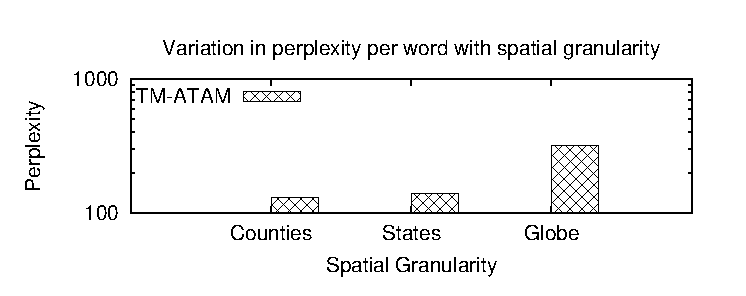
\epsfig{file=gnuplot/perplexity/perplexityGeographic,width=0.42\textwidth}
\caption{Variation in performance of \tmatam with geographic granularity over regions. "States" and "Counties" correspond to first and second level administrative divisions.}
\label{fig:perplexitySpatial}
\end{figure}
We examine two different choices for the geographic 
granularity i.e. \emph{states} and \emph{counties} which correspond to
first and second level administrative divisions. \footnote{\url{https://en.wikipedia.org/wiki/Table_of_administrative_divisions_by_country}}
While \tmatam can be instantiated at varying granularities of space, 
learning accurate ailment distributions requires a certain minimum number 
of tweets.  Selecting larger 
than optimal sized regions would introduce errors 
into the prediction algorithm. Choice of geographic granularity is non-trivial.
Predicted perplexity in counties is lower, hence better, than perplexity at the level of states as shown in Figure~\ref{fig:perplexitySpatial}.
We attribute this result to the fact that tweets from smaller regions show less diversity in topics.
\subsubsection{Temporal Granularity}
\begin{figure}[t!]
\centering
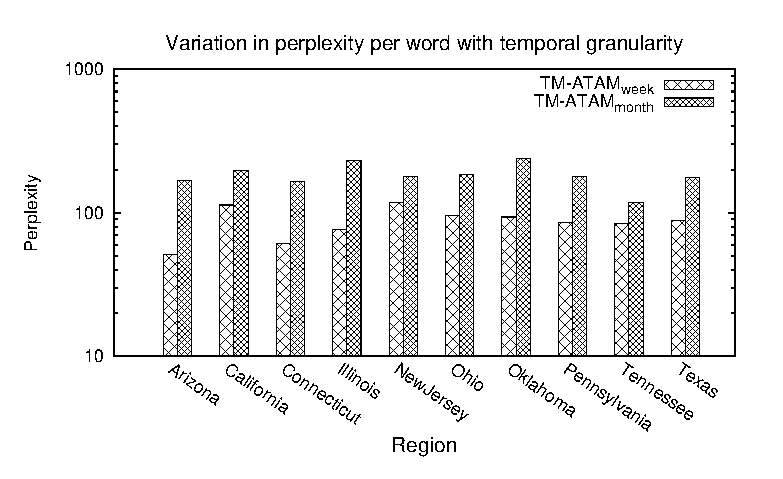
\epsfig{file=gnuplot/perplexity/perplexityTemporalUS,width=0.45\textwidth}
\caption{Variation in perplexity achieved by \tmatam at different 
temporal granularities. Results for top-10 social media active regions.}
\label{fig:perplexityTemporalUS}
\end{figure}
\begin{figure}[b!]
\centering
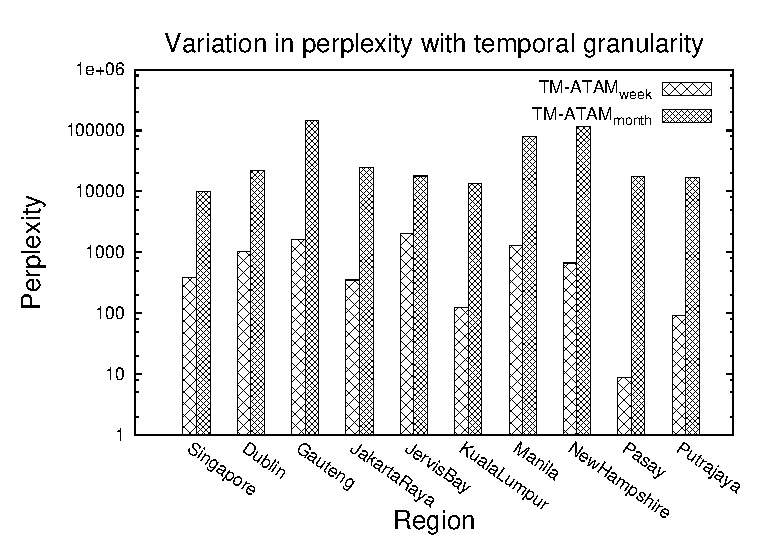
\epsfig{file=gnuplot/perplexity/perplexityTemporalNonUS,width=0.45\textwidth}
\caption{Variation in perplexity achieved by \tmatam at different 
temporal granularities. Results for top-10 non-US active regions.}
\label{fig:perplexityTemporalNonUS}
\end{figure}
We examine two different temporal granularities, \emph{months} 
and \emph{weeks}. Analogous to geographic granularity, choice of temporal 
granularity should not be too fine or too coarse. We show performance 
of \tmatam on time granularities in Figures~\ref{fig:perplexityTemporalUS} 
and \ref{fig:perplexityTemporalNonUS}. 
This is also attributed to the fact that prediction of health topics in smaller temporal granularity is more accurate as health topics do not transform by a substantial amount in shorter periods.
\subsubsection{Distance Measures}
The obtained \change-boundary depends on the choice of distance measure $m$.
We conduct experiments with two different measures, namely, Bhattacharya
Distance and Cosine Similarity. We convert the latter to a distance
measure $d=\sqrt{2-2\times cos}$ where $cos$ is the cosine similarity.
For each measure, we compute perplexity over \emph{pre} and \emph{post} 
time intervals. Results are shown in Figures~\ref{fig:perplexityMeasureUS} 
and \ref{fig:perplexityMeasureNonUS}. On an average over regions, 
Bhattacharya Distance outperforms Cosine Similarity. We observed that number of 
tweets at a given time granularity $t$ may affect the performance of Cosine Similarity. This may
happen even after normalizing the topic vectors into unit-length as some of the topics may not even get instantiated.
\begin{figure}[t!]
\centering
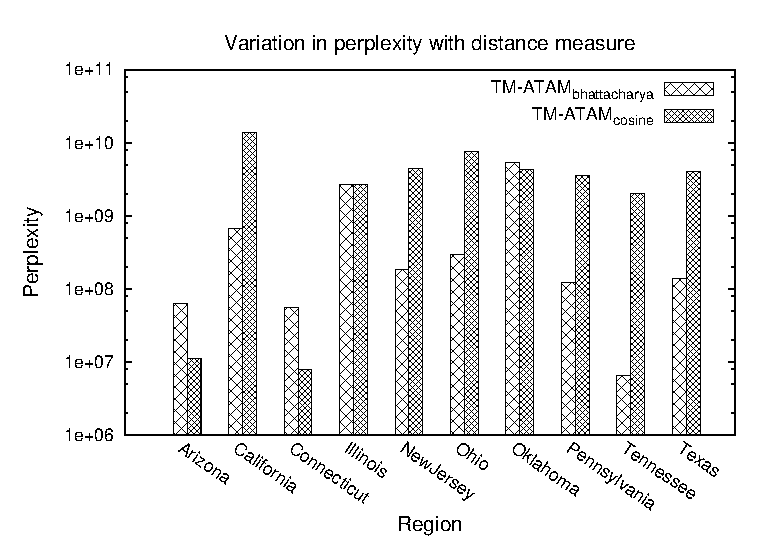
\epsfig{file=gnuplot/perplexity/perplexityMeasureUS.eps,width=0.45\textwidth}
\caption{Variation in perplexity achieved by \tmatam with different 
distance measures. Results computed over top-10 active U.S. regions.}
\label{fig:perplexityMeasureUS}
\end{figure}
\begin{figure}[t!]
\centering
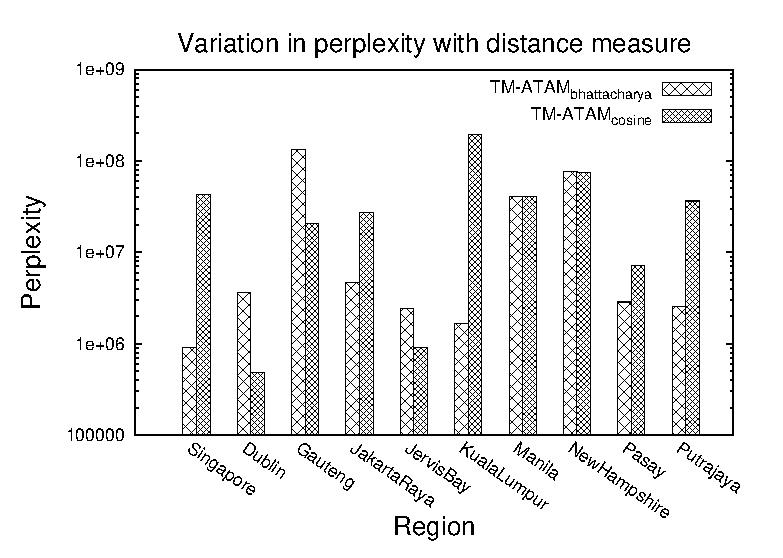
\epsfig{file=gnuplot/perplexity/perplexityMeasureNonUS.eps,width=0.45\textwidth}
\caption{Variation in perplexity achieved by
TM–ATAM with different distance measures. Results
computed over top-10 non-US active regions.}
\label{fig:perplexityMeasureNonUS}
\end{figure}
\subsection{Qualitative Analysis of \tmatam}
\label{subsec:qualitative}
\subsubsection{\changes}
\label{subsubsec:season}
The central idea in TM–ATAM is to identify \changes, i.e.,
time intervals that exhibit homogeneous ailment distributions, as well
as transitions between them.
A natural question that emerges is {\em how and why} ailments
differ across \change boundaries. In Figures 13 and 14
we show the sharpest change point, representing the strongest
transition, for the top-10 US and
non-US regions respectively. Those points can be explained with weather
changes in those regions. For example, Texas can be explained with a
drop in temperature while Jervis Bay can be explained by an increase in
rainfall. Dublin sees its lowest temperature in the November period.
Singapore and Manila have very similar weather conditions and exhibit
the same change point. A deeper look at these transitions would provide
more insights.
\begin{figure}[b!]
\centering
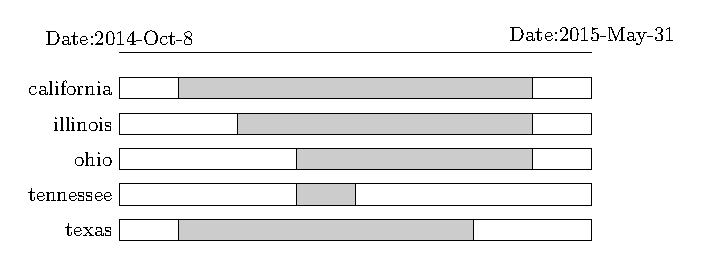
\includegraphics[width=0.45\textwidth]{tikz/seasons.pdf}
\caption{Monthly \change boundaries for top-10  active U.S. regions.}
\label{fig:seasonBoundary:US}
\end{figure}
\begin{figure}[b!]
\centering
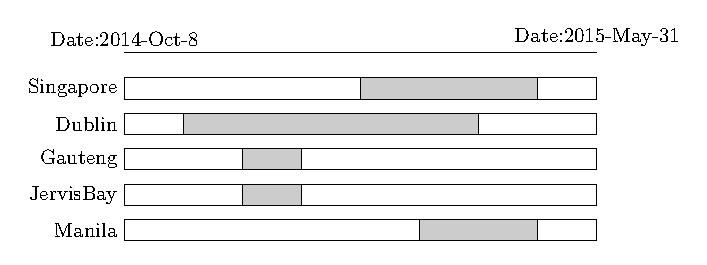
\includegraphics[width=0.45\textwidth]{tikz/seasonsNonUS.pdf}
\caption{Monthly \change boundaries for top-10 active non-U.S. regions.}
\label{fig:seasonBoundary:NonUS}
\end{figure}
\begin{table*}[t!]
\centering
\caption{$M_{full}$ transitions for California (threshold: $0.815$)}
\label{tab:fulltransitionCalifornia}
\begin{tabular}{|c|c|c|l|} \hline
Transition Type & From Topic&To Topic&Weight\\ \hline
One-Way Transitions & smoking/junkies/drugs/cigarettes & respiratory diseases&  2.70\\ 
 & depression/complaining/cursing/slangs/self-pity &  joint pains/body pains&  3.25\\
 \hline\end{tabular}
\end{table*}
\subsubsection{Topic Transitions}
Entry $m_{ij}$ in the transition parameter matrix $M$ produced by
\tmatam, shows the degree that topic $z_i$ will contribute to topic $z_j$
in the following \change. We analyze 3 kinds of transition matrices
corresponding to our setting: \textit{intra-\change}: $M_{pre}$, $M_{post}$
and  \textit{full-time-period}: $M_{full}$ .
We adapt the threshold used in \cite{DBLP:conf/kdd/WangAB12} to our settings:
\begin{equation}
Threshold  = \mu + 2\times\sigma_{non-diagonal}
\end{equation}
Here $\mu$ is the mean of the corresponding transition matrix. $\sigma_{non-diagonal}$ is the standard deviation of non-diagonal entries. We choose this threshold because 95.45\% of the values lie within two standard deviations of the mean.\footnote{\url{https://en.wikipedia.org/wiki/68-95-99.7_rule}}
We identify three kinds of 
interesting transitions based on the threshold defined in~\cite{DBLP:conf/kdd/WangAB12}:
\begin{itemize}
 \item Self transitions: Diagonal entries above threshold
 \item Symmetric Transitions: Both $m_{ij}$ and $m_{ji}$ is higher than threshold
 \item One-Way Transitions: Only one of $m_{ij}$ and $m_{ji}$ is higher than threshold
\end{itemize}
\begin{table}[t!]
\centering
\caption{$M_{full}$: California}
\label{tab:statsCalifornia}
\begin{tabular}{|c|l|} \hline
\#tweets & 55475 \\ \hline
$\mu_{full}$ & 0.015\\ \hline
$\sigma_{non-diagonal}$& 0.4\\ \hline
$\mu_{diagonal}$ & -0.002 \\ \hline
Threshold & 0.015 + $2\times0.4$ = 0.815 \\ 
 \hline\end{tabular}
\end{table}
Mean of diagonal entries is the quantification of how stable the 
transitions are and standard deviation of non-diagonal entries is 
the quantification of how much the topics fluctuate in the given 
time granularity. Let mean be denoted by $\mu$ and standard deviation 
be denoted by $\sigma$ for further discussion
\begin{table*}[t!]
\centering
\caption{$M_{full}$ (Threshold: 0.45) Transitions for Kuala Lumpur}
\label{tab:transitionKualaLumpur}
\begin{tabular}{|c|c|c|l|} \hline
Type &From Topic&To Topic&Weight\\ \hline
One-Way Transition& Heart Disease/Blood Pressure & Coughing/runny nose/watery eyes&0.85\\
 & Brain Disorder & Body pains/Weight Loss&0.599\\
 &Urinary Infection/Intestine/Tract & Stomach Pain/Blood Pressure&0.51\\
\hline\end{tabular}
\end{table*}
Table \ref{tab:statsCalifornia} summarizes the essential statistics 
of \textit{$M_{full}$} of California. As can be observed 
from 4th entry, $\mu_{diagonal}$ in Table \ref{tab:statsCalifornia} 
is almost 0 and this is intuitive because health topics transition a lot 
between \changes. Table~\ref{tab:fulltransitionCalifornia} lists 
interesting one-way health topic transitions observed in California for the full time period. Self-Transitions are hard to find
in \textit{full} time periods as topics change randomly. 
\begin{table*}[t!]
\centering
\caption{$M_{pre}$ transitions in Arizona (threshold: $0.035$)}
\label{tab:fulltransitionArizona}
\begin{tabular}{|c|c|c|l|} \hline
Transition Type & From Topic&To Topic&Weight\\ \hline
Self-Transition & Stomach Infection & Stomach Infection& 0.064\\ 
  &Headache &Headache& 0.09\\ \hline
Symmetric-Transition & Stomach Infection & Headache & 0.06\\ 
& Headache & Stomach Infection & 0.09\\
 & Stomach Infection & Pneumonia & 0.05\\ 
& Pneumonia & Stomach Infection & 0.04\\ 
 \hline\end{tabular}
\end{table*}	
\begin{table}[b!]
\centering
\caption{Transitions Stats for Kuala
Lumpur}
\label{tab:transitionStatsKualaLumpur}
\begin{tabular}{|c|l|} \hline
Statistic & Value \\ \hline
$\mu_{diagonal}$  $M_{full}$ &0.0025\\ \hline
$\mu_{diagonal}$ $M_{post}$ & 0.01 \\ \hline
$\mu_{diagonal}$  $M_{pre}$ &  0.024\\ \hline
$\sigma_{non-diagonal}$ $M_{full}$ & 0.09 \\ \hline
$\sigma_{non-diagonal}$ $M_{post}$& 0.068\\ \hline
$\sigma_{non-diagonal}$ $M_{pre}$& 0.018\\
 \hline\end{tabular}
\end{table}
\begin{table}[b!]
\centering
\caption{$M_{pre}$ (Threshold: 0.039) and $M_{post}$ (Threshold: 0.13) Transitions for Kuala Lumpur}
\label{tab:transitionKualaLumpurprepost}
\begin{tabular}{|c|c|c|l|} \hline
Type &From Topic&To Topic&Weight\\ \hline
Self Transition $M_{pre}$ & headache & headache& 0.19 \\ \hline
Self Transition $M_{post}$& body pain& body pain& 0.228\\ 
\hline\end{tabular}
\end{table}
Further, we analyze $M_{pre}$, $M_{post}$ and $M_{full}$ of Kuala\\
 Lumpur. Various statistics are summarized in Table~\ref{tab:transitionStatsKualaLumpur}.\\
 $\mu_{diagonal}$ is consistently higher for $M_{pre}$ and $M_{post}$ than $M_{full}$. $\sigma_{non-diagonal}$ is higher for
 $M_{full}$ than both \textit{intra-\change} transition matrices. These statistics go on to 
show that health topics do not drastically change and are coherent within 
the same \change and transform into one another a lot across the 
\changes. This further re-instates this fact that it is 
more sensible to model topic transition matrices within the same
\change and update them once the \change has ended. Further, 
we analyze the interesting self transitions of \textit{intra-\change}
($M_{pre}$ and $M_{post}$) and one-way transitions of $M_{full}$.
Arizona transitions are summarized in Table \ref{tab:fulltransitionArizona} and Kuala-Lumpur transitions are summarized in Tables
\ref{tab:transitionKualaLumpur} and \ref{tab:transitionKualaLumpurprepost}.


\section{Related Work}
\label{sec:relwork}
Proliferation of social media platforms such as \emph{Twitter},
\emph{pinterest}, \emph{facebook}, \emph{tumblr} has led to their
application to a wide array of tasks including mental health
assessment~\cite{twitter:anorexia,twitter:violence,twitter:mental}, 
inferring political affiliation~\cite{twitter:elec,twitter:elec2,twitter:elec3,twitter:elec4},
brand perception~\cite{twitter:brand,twitter:brand2} etc.

Social media, especially Twitter, are good sources of personal
health~\cite{twitter:health,twitter:health2,twitter:health3,twitter:health4}.
Previous studies on public health surveillance have attempted to
uncover ailment topics on online
discourse~\cite{DBLP:conf/nips/ChemuduguntaSS06,atam2} or model the
evolution of general topics~\cite{DBLP:conf/kdd/WangAB12}. In this
paper, we combine the best of both worlds which leads to the discovery
of \emph{disease-\changes} for social-media active regions. We model
the evolution of diseases within \changes and obtain significant
improvement over the previous state of the art for public health
surveillance using social media.

We propose TM-ATAM, an approach that builds on the previously proposed
TM-LDA for modeling general topic evolution over
time~\cite{DBLP:conf/kdd/WangAB12}. Just like TM-LDA, TM-ATAM learns
topic transitions over time and not topic trends. Such transitions the
purpose of answering questions such as people talk about fever before
talking about stomach ache. Other complementary approaches that learn
the dynamicity of word distributions or topic trends have been
proposed. That is the case of~\cite{DBLP:conf/icml/BleiL06} that
models topic evolution over time as a discrete chain-style process
where each piece is modeled using
LDA. In~\cite{DBLP:conf/kdd/WangM06}, the authors propose a method
that learns changing word distributions of topics over time and
in~\cite{DBLP:conf/icdm/LinMHJD11}, the authors leverage the structure
of a social network to learn how topics temporally evolve in a
community. Finally, in~\cite{DBLP:conf/wsdm/SahaS12}, Non-negative
Factorization is used for learning topic trends. Exploring the
applicability of those complimentary approaches to the evolution of
health topics in tweets, is a promising research direction.




\section{Conclusion and Future Work}
\label{sec:conclusion}
In this paper we study methods to uncover disease distributions hidden
within social media.  We propose a granularity-based model to conduct
region-specific analysis that leads to the identification of time
intervals characterizing homogeneous disease discourse, per region.
We achieve this by comparing ailment distributions for consecutive
time periods within each region.  We term such periods as
\emph{\changes}.  Subsequently we model the temporal evolution of
diseases within each \emph{\changes} and attempt to predict ailments
ahead of time.  The fine-grained nature of our model results in
significant improvements in modeling and predicting transitions of
health-related tweets over state of the art methods.  We envisage a
use case where our disease predictions can replace existing solutions
for syndromic surveillance of diseases that are both costly and time
consuming.


\bibliographystyle{unsrt}
\bibliography{./bib/references}

% Proforma: table (normal)
% \comment{
% 	\begin{table}
% 	\centering
% 	\caption{Frequency of Special Characters}
% 	\begin{tabular}{|c|c|l|} \hline
% 	Non-English or Math&Frequency&Comments\\ \hline
% 	\O & 1 in 1,000& For Swedish names\\ \hline
% 	$\pi$ & 1 in 5& Common in math\\ \hline
% 	\$ & 4 in 5 & Used in business\\ \hline
% 	$\Psi^2_1$ & 1 in 40,000& Unexplained usage\\
% 	\hline\end{tabular}
% 	\end{table}
% }	

% Proforma: table (wide)
% \comment{
% 	\begin{table*}
% 	\centering
% 	\caption{Some Typical Commands}
% 	\begin{tabular}{|c|c|l|} \hline
% 	Command&A Number&Comments\\ \hline
% 	\texttt{{\char'134}alignauthor} & 100& Author alignment\\ \hline
% 	\texttt{{\char'134}numberofauthors}& 200& Author enumeration\\ \hline
% 	\texttt{{\char'134}table}& 300 & For tables\\ \hline
% 	\texttt{{\char'134}table*}& 400& For wider tables\\ \hline\end{tabular}
% 	\end{table*}
% }

% Proforma: figure (normal)
% \comment{
% 	\begin{figure}
% 	\centering
% 	\epsfig{file=fly.eps}
% 	\caption{A sample black and white graphic (.eps format).}
% 	\end{figure}
% }

% Proforma: figure (wide)
% \comment{
% 	\begin{figure*}
% 	\centering
% 	\epsfig{file=flies.eps}
% 	\caption{A sample black and white graphic (.eps format)
% 	that needs to span two columns of text.}
% 	\end{figure*}
% }
% 
% % Proforma: theorem 
% \comment{
% 	\newtheorem{theorem}{Theorem}
% 	\begin{theorem}
% 	Let $f$ be continuous on $[a,b]$.  If $G$ is
% 	an antiderivative for $f$ on $[a,b]$, then
% 	\begin{displaymath}\int^b_af(t)dt = G(b) - G(a).\end{displaymath}
% 	\end{theorem}
% }
% 
% % Proforma: definition
% \comment{
% 	\newdef{definition}{Definition}
% 	\begin{definition}
% 	If $z$ is irrational, then by $e^z$ we mean the
% 	unique number which has
% 	logarithm $z$: \begin{displaymath}{\log e^z = z}\end{displaymath}
% 	\end{definition}
% }


\end{document}
